\begin{frame}
    \begin{center}
        {\huge 4.2: \textbf{Numerical Results}}\\
        {\normalsize\noindent (Trajectory Optimization of Gliding Hypersonic Systems)}
    \end{center}
\end{frame}

\begin{frame}{Numerical Results: Trajectory Optimization}
    \footnotesize
    \visible<1->{We want to \textbf{optimally control} a gliding hypersonic system,}
    \begin{columns}
        \begin{column}{0.55\textwidth}
            \visible<5->{
            \begin{graybox}{Optimal Control Problem (\textcolor{red}{Costly to Solve!})}
                \visible<6->{
                Find $\vu^*(t)$ that minimizes the cost functional,}
                \vspace*{-0.1in}
                \begin{align*}
                    \visible<7->{
                    \min_{\vu}\:\cJ(\vu;\vp) &= \varphi(\vs(t_f),t_f) + \int_{t_0}^{t_f} \ell(\vs(t),\vu(t),t;\vp)dt}\\
                    \visible<8->{
                    \vspace*{-0.02in}
                    \text{s.t.}\quad \dot{\vs} &= \vf\left(\vs,\vu;\vp\right)\rightarrow\text{{\tiny EOMs}}}\\
                    \visible<9->{
                    \vzero &= \vPsi_0\left(\vs(t_0),t_0;\vp\right)\rightarrow\text{{\tiny deployment conditions}}}\\
                    \visible<10->{
                    \vzero &= \vPsi_f\left(\vs(t_f),t_f;\vp\right)\rightarrow\text{{\tiny terminal conditions}}}
                \end{align*}
                \visible<11->{
                We need efficient \textbf{real-time solutions} via,
                \begin{equation*}
                    \vu^*(t) = \arg\min_{\vu}\left\{\ell\left(\vs,\vz_{\text{HF}},\vu\right) + \frac{\partial V}{\partial\vs}^\top \vf\left(\vs,\vu;\vp\right)\right\}
                \end{equation*}}
            \end{graybox}}
        \end{column}
        \begin{column}{0.45\textwidth}
            \visible<2->{
            \begin{graybox}{Guidance}
                \centering
                \visible<3->{
                \begin{figure}
                    \centering
                    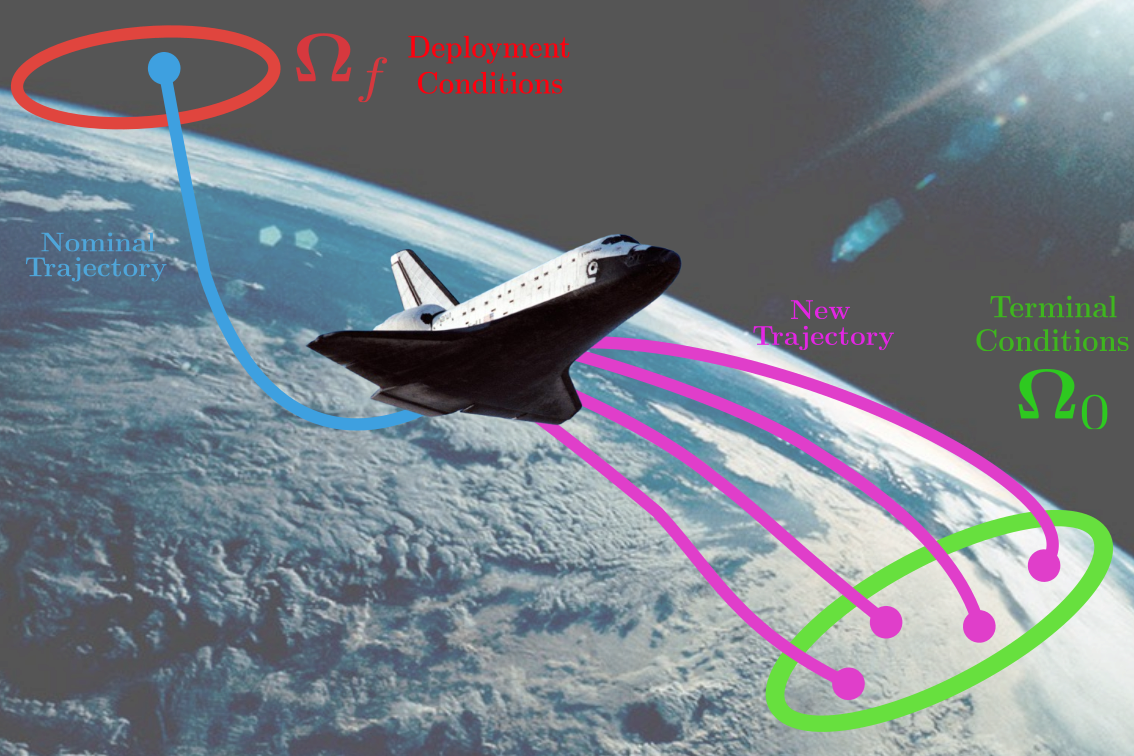
\includegraphics[width=0.9\textwidth]{../figs/guidance/guidance.png}
                \end{figure}}
                \vspace*{-0.1in}
                \visible<4->{
                We need \textbf{on-board real-time guidance!}}
            \end{graybox}}
        \end{column}
    \end{columns}
    \begin{center}
        {\tiny $\vs$: state vector, $\vu$: control vector, $\vp$: system parameters, $\cJ$: cost functional, $\varphi$: terminal cost, $\ell$: running cost, $\vf$: system dynamics, $\vPsi_0$: initial constraints, $\vPsi_f$: terminal constraints}
    \end{center}
\end{frame}

\begin{frame}{Numerical Results: Trajectory Optimization}
    \footnotesize
    \visible<1->{\textbf{Sparse physics-informed} learning of governing \textbf{value function},}
    \vspace*{-0.1in}
    \begin{columns}
        \begin{column}{0.5\textwidth}
            \visible<2->{
            \begin{graybox}{Polynomial Approximation}
                \begin{itemize}
                    \item<3-> \textbf{Input}: $\vx=\left(x_1,x_2,\dots,x_d\right)^\top\in\mathbb{R}^{d}$
                    \item<4-> \textbf{Maximum basis order}: $O$
                    \item<5-> \textbf{Number basis}: $m = \begin{pmatrix}
                        d + O\\
                        d
                    \end{pmatrix} = \frac{(d + O)!}{d!O!}$
                    \item<6-> \textbf{Index}: $\valpha_i = \left(\alpha^i_1,\dots,\alpha^i_d\right)\in\mathbb{N}^d$
                    \vspace*{-0.1in}
                    \begin{equation*}
                        \alpha_1 + \alpha_2 + \dots + \alpha_d \leq O
                        \vspace*{-0.1in}
                    \end{equation*}
                    \item<7-> \textbf{For example} $d=2$, $O=2$:
                    \vspace*{-0.1in}
                    \begin{columns}
                    \begin{column}{0.3\textwidth}
                        \visible<8->{
                        \begin{equation*}
                        \mathbf{I} = \begin{pmatrix}
                            0 & 0\\
                            1 & 0\\
                            0 & 1\\
                            2 & 0\\
                            1 & 1\\
                            0 & 2
                        \end{pmatrix}
                        \vspace*{-0.1in}
                        \end{equation*}}
                    \end{column}
                    \hspace*{-0.4in}
                    \begin{column}{0.3\textwidth}
                        \visible<9->{
                        \begin{align*}
                            \Phi &= \left\{\phi_i(\vx)\right\}_{i=1}^{m}\\
                            &= \left\{1, x_1, x_2, x_1^2, x_1x_2, x_2^2\right\}
                            \vspace*{-0.1in}
                        \end{align*}}
                    \end{column}
                    \vspace*{-0.1in}
                    \end{columns}
                \end{itemize}
            \end{graybox}}
        \end{column}
        \hspace*{-0.1in}
        \begin{column}{0.5\textwidth}
            \visible<10->{
            \begin{graybox}{Optimal Control Policy}
                \visible<11->{
                Value function parametrization,
                \begin{equation*}
                    V(\vx,t) = \sum_{i=1}^{m}\redTheta_i(t)\phi_i(\vx)
                \end{equation*}
                \vspace*{-0.1in}
                Learn \textbf{optimal parameters} $\redvTheta^*(t)$ such that,}
                \visible<12->{
                \begin{equation*}
                    \vu^*(t) = \arg\min_{\vu}\left\{\ell(\vs,\vu,\vp) + \frac{\partial V}{\partial\vs}^\top\vf\left(\vs,\vu;\vp\right)\right\}
                \end{equation*}}
            \end{graybox}}
        \end{column}
    \end{columns}
\end{frame}

\begin{frame}{Numerical Results: Trajectory Optimization}
    \footnotesize
    \visible<1->{Minimize \textbf{expected} performance over the \textbf{optimality conditions},}
    \begin{columns}
        \begin{column}{0.7\textwidth}
            \visible<1->{
            \begin{graybox}{Parameters: BCs $\vtheta$ and Model Parameters $\vxi$}
                \only<1>{
                    \begin{figure}
                        \centering
                        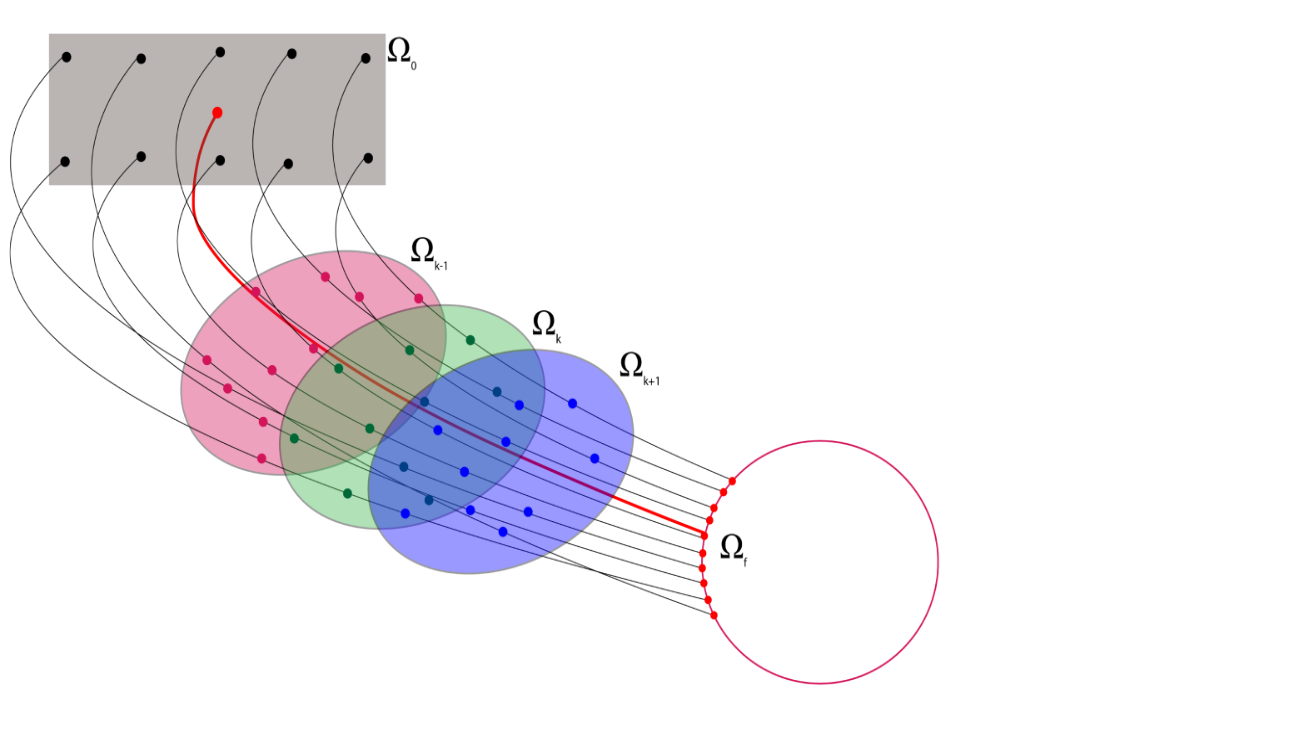
\includegraphics[width=0.9\textwidth]{../figs/guidance/parameters_1.png}
                    \end{figure}}
                \only<2>{
                    \begin{figure}
                        \centering
                        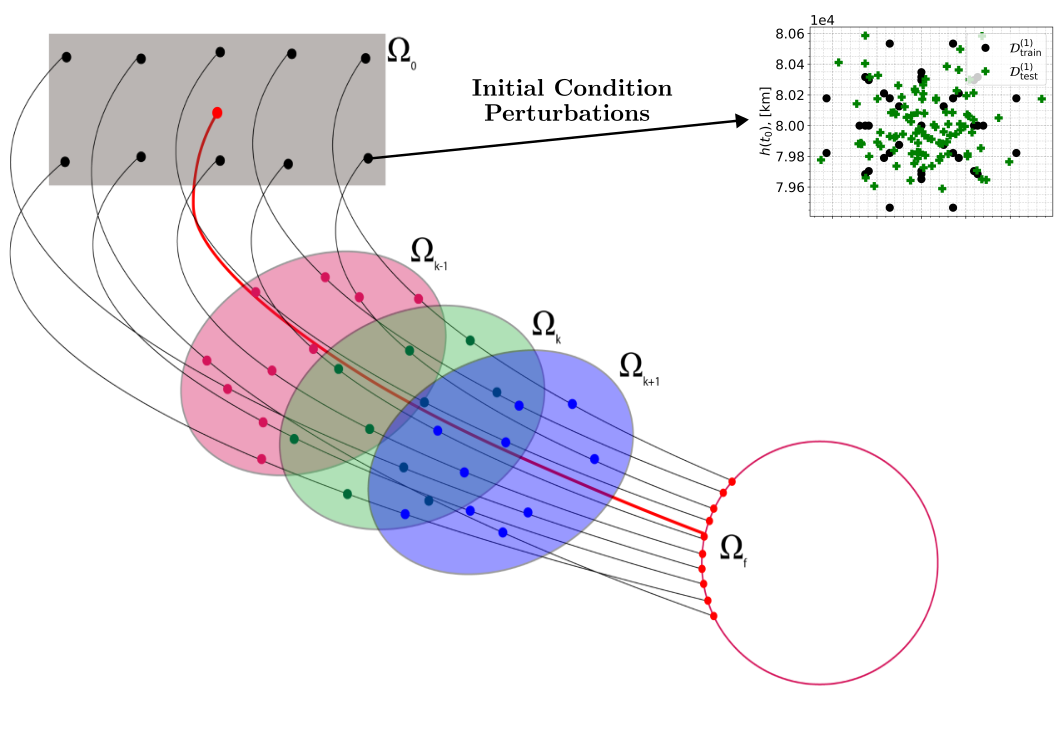
\includegraphics[width=0.9\textwidth]{../figs/guidance/parameters_2.png}
                    \end{figure}}
                \only<3>{
                    \begin{figure}
                        \centering
                        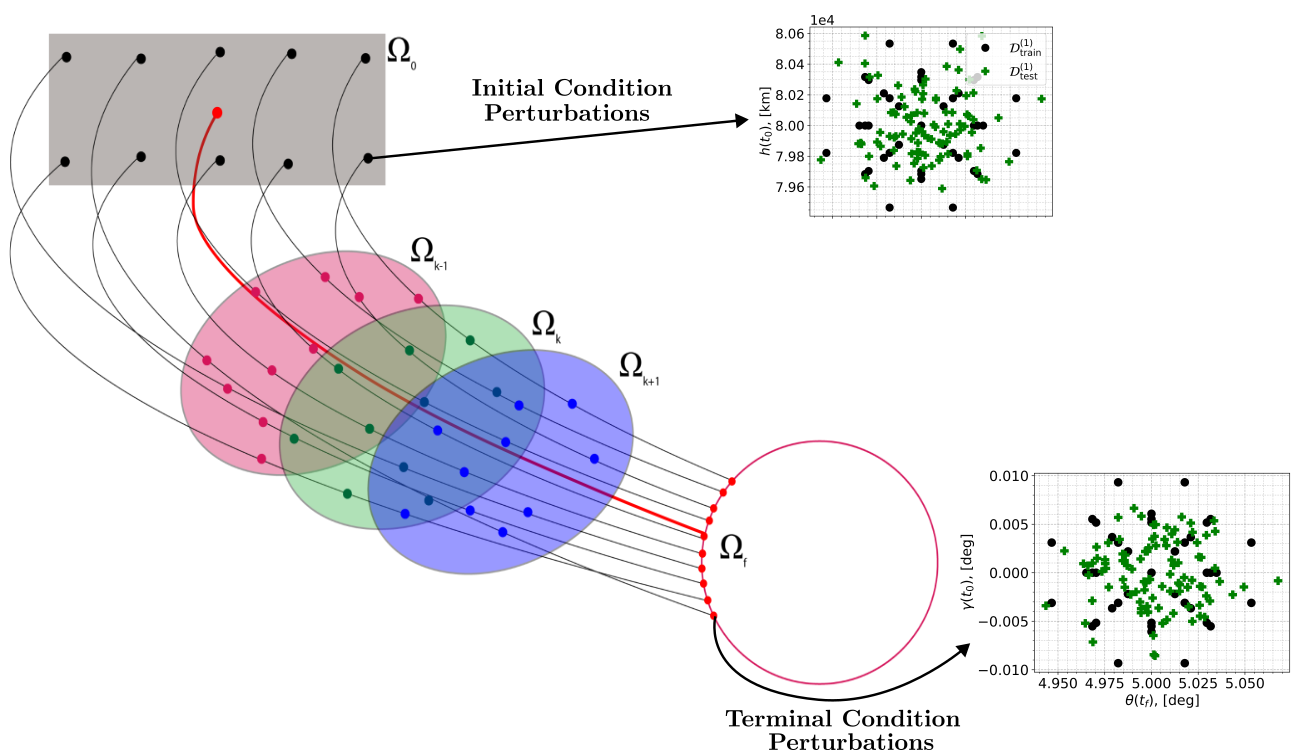
\includegraphics[width=0.9\textwidth]{../figs/guidance/parameters_3.png}
                    \end{figure}}
                \only<4>{
                    \begin{figure}
                        \centering
                        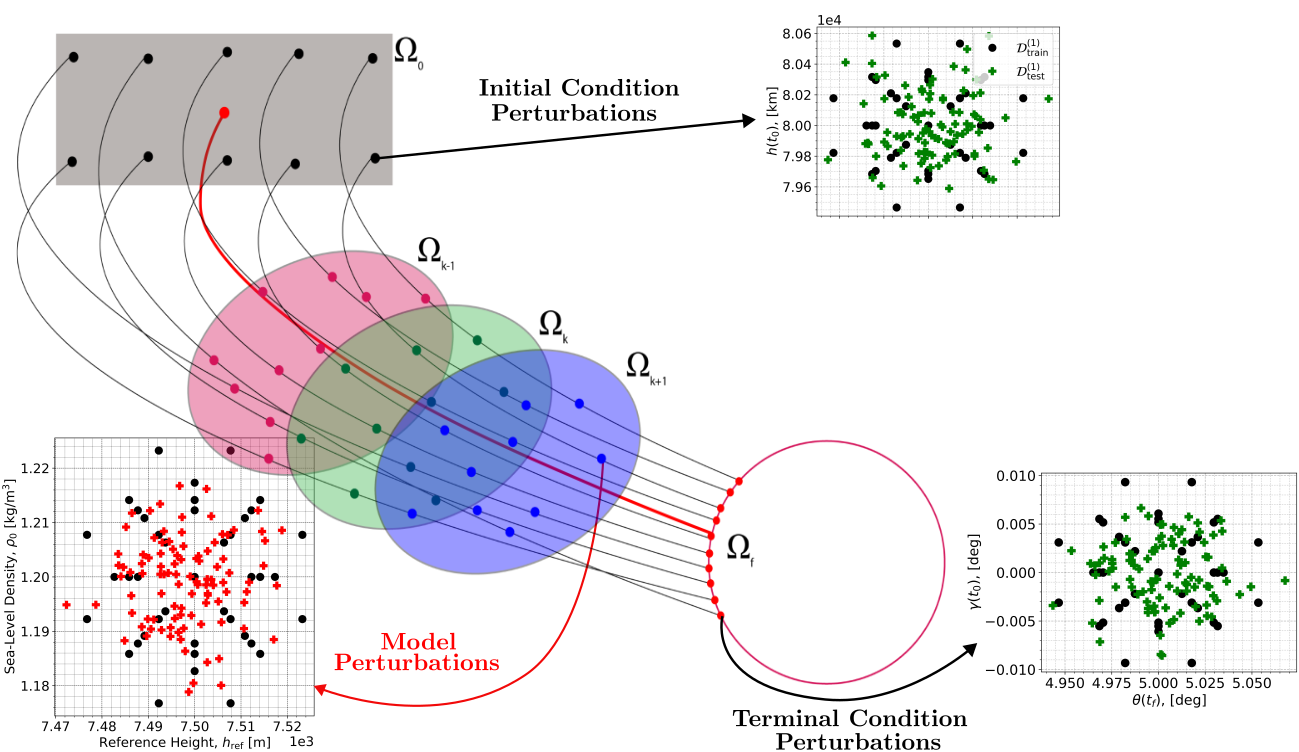
\includegraphics[width=0.9\textwidth]{../figs/guidance/parameters_4.png}
                    \end{figure}}
                \only<5->{
                    \begin{figure}
                        \centering
                        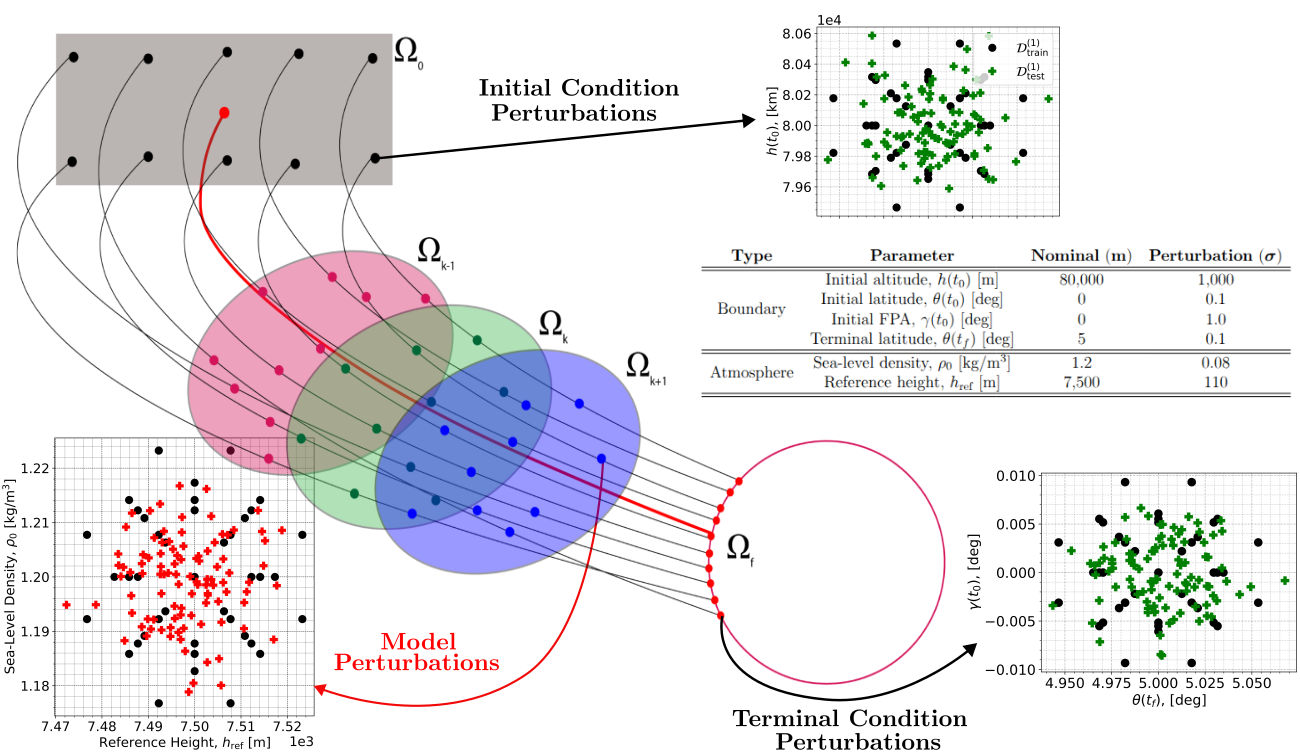
\includegraphics[width=0.9\textwidth]{../figs/guidance/parameters_5.png}
                    \end{figure}}
            \end{graybox}}
        \end{column}
        \begin{column}{0.4\textwidth}
            \visible<6->{
            \begin{graybox}{Indirect OCP Solutions}
                \begin{figure}
                    \centering
                    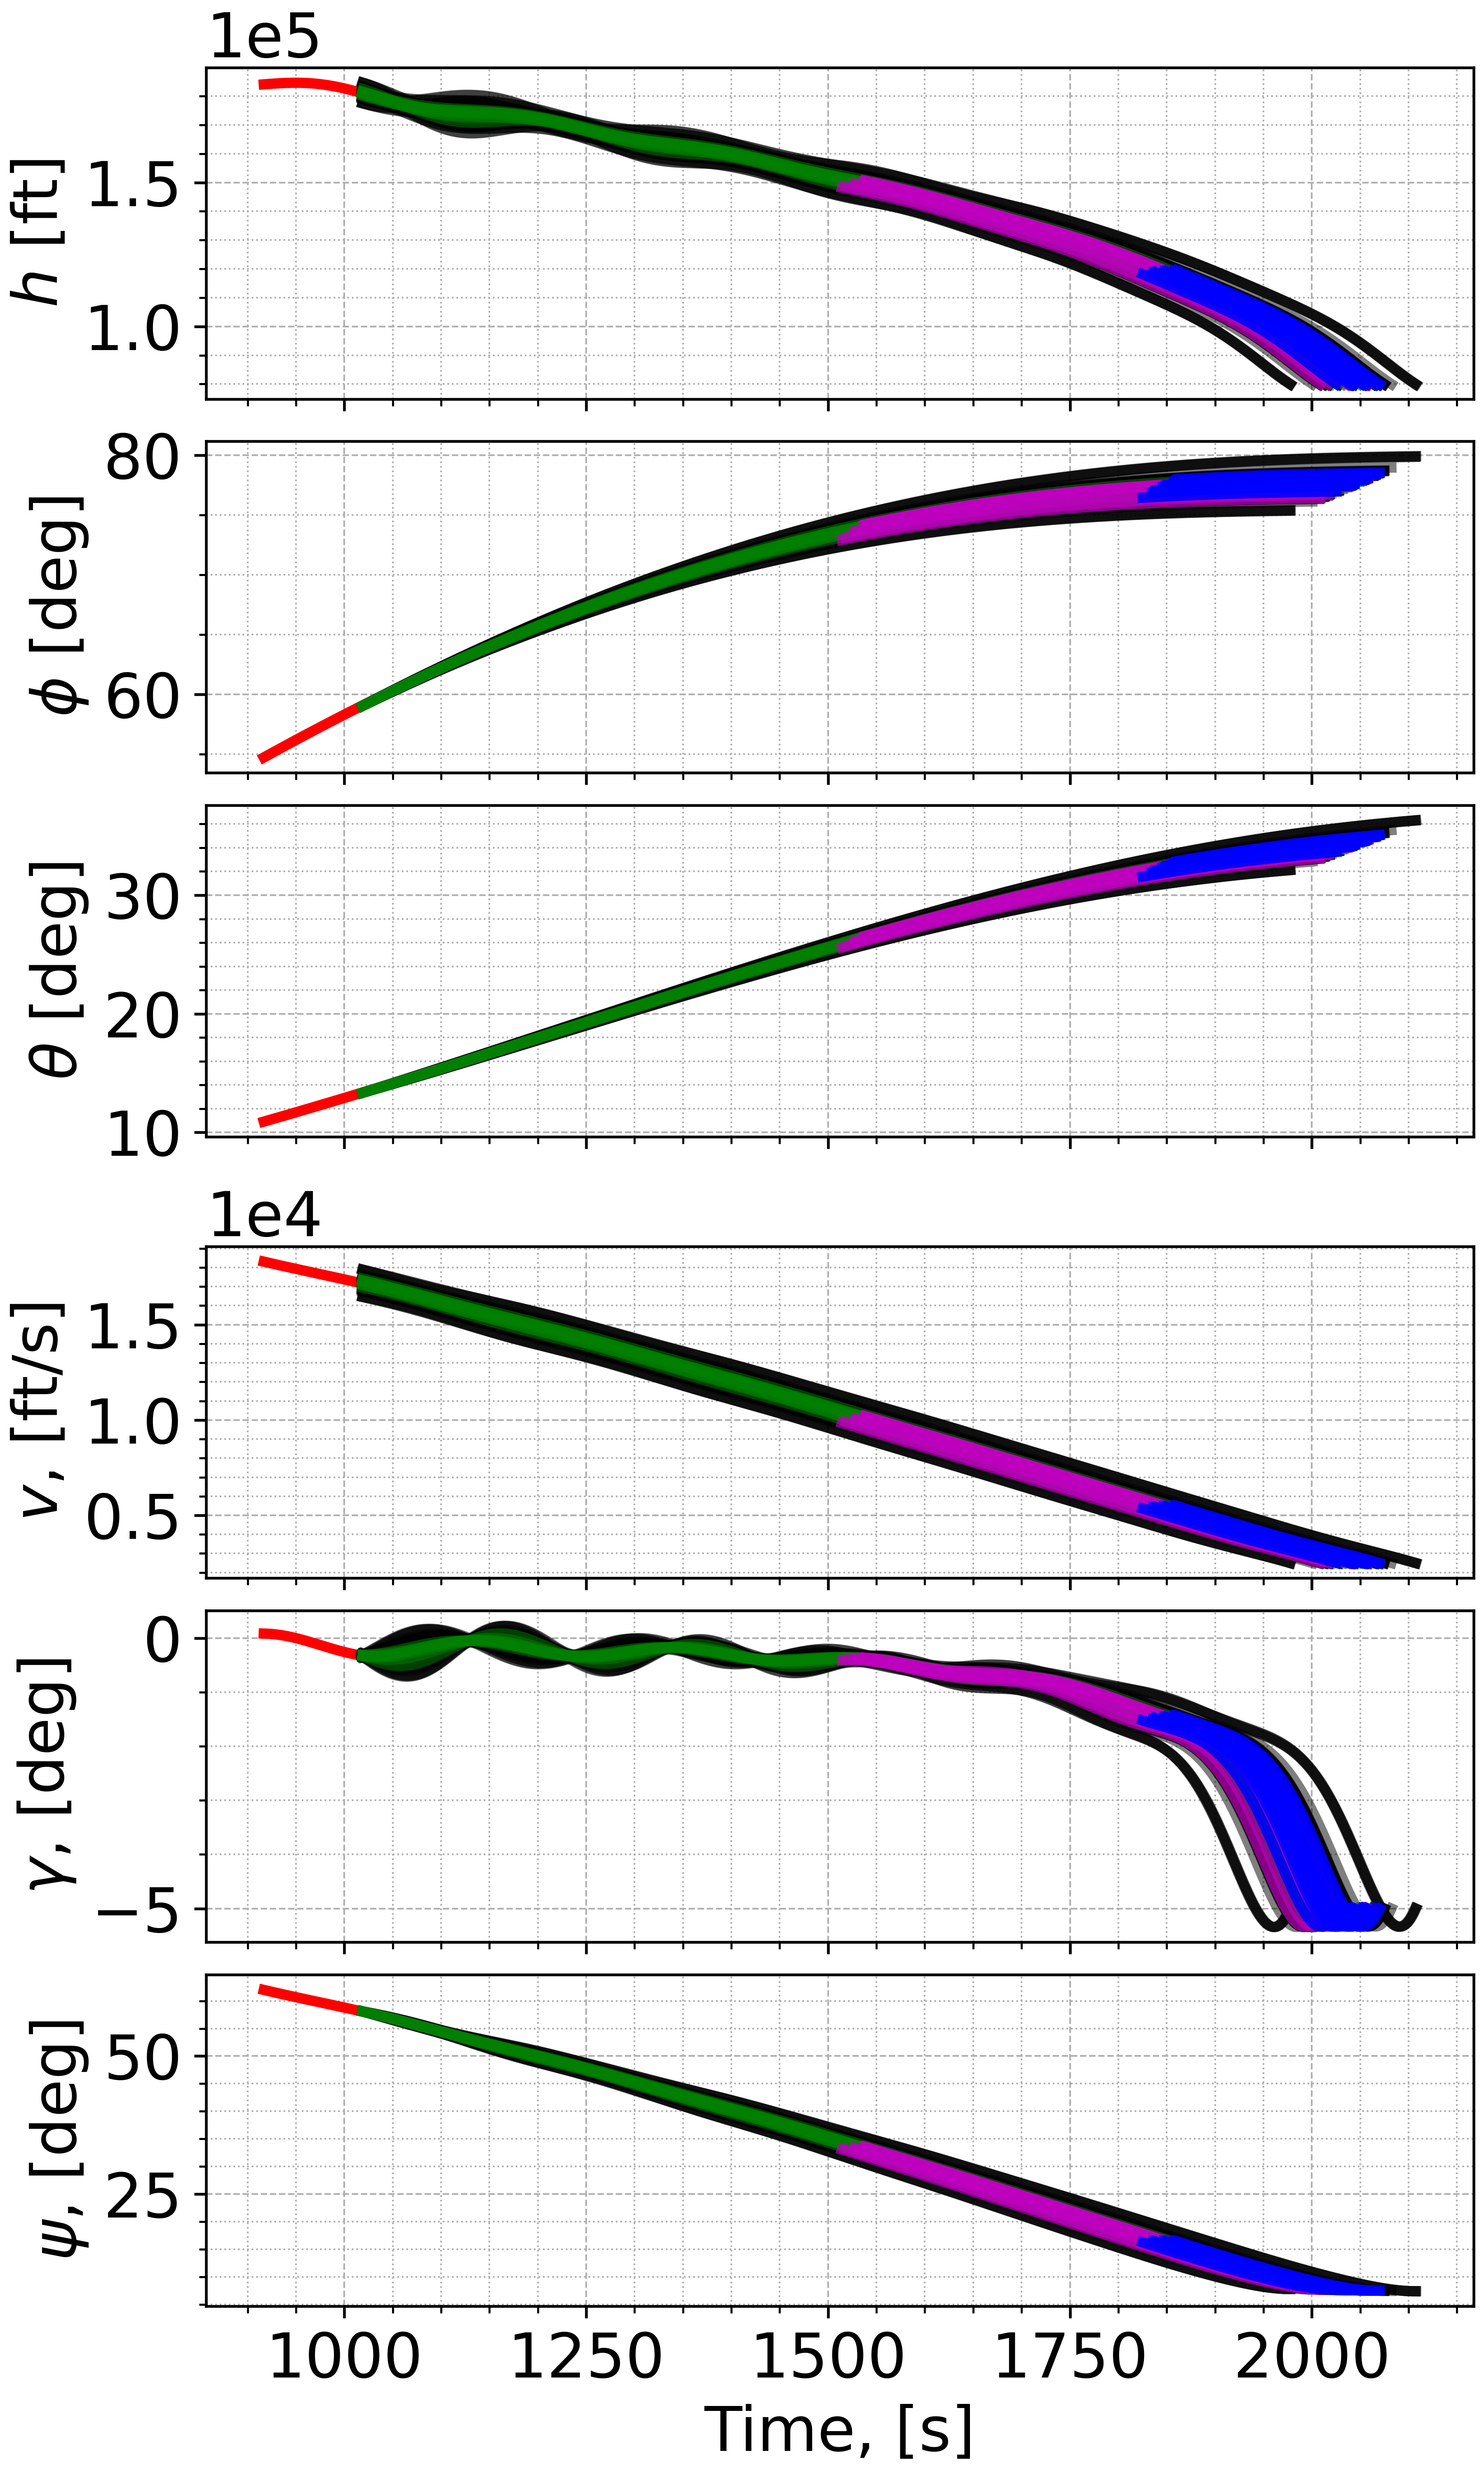
\includegraphics[width=0.7\textwidth]{../figs/guidance/space_shuttle_states.png}
                \end{figure}
            \end{graybox}}
        \end{column}
    \end{columns}
\end{frame}

\begin{frame}{Numerical Results: Trajectory Optimization}
    \footnotesize
    \visible<1->{The \textbf{impossible trinity of optimal control} is \textbf{quantified} as,}
    \begin{columns}
        \visible<1->{
        \begin{column}{0.4\textwidth}
            \begin{figure}
                \centering
                
\includegraphics[width=0.9\textwidth]{../../Chapter-1/Figures/itoc.png}
            \end{figure}
        \end{column}}
        \begin{column}{0.6\textwidth}
            \begin{itemize}
                \visible<2->{
                \item \textbf{Accuracy}: normalized root mean square error (NRMSE),
                \begin{equation*}
                    e\left(y_{\text{HF}},y\right) = \frac{1}{\Delta y}\sqrt{\frac{1}{n_p}\sum_{k=0}^{p-1}\left(y_{\text{HF}}(t_k) - y(t_k)\right)^2}\times 100\%
                \end{equation*}}
                \visible<3->{
                \item \textbf{Efficiency}: acceleration $\mathcal{A}$, and compression ratio $\cC$,
                \begin{equation*}
                    \mathcal{A} = \frac{\cT_{\text{HF}}(\vx,t)}{\cT_{\cM}(\vx,t)},\quad \cC = \frac{\left|\hat{\Phi}\right|}{\left|\Phi\right|}
                \end{equation*}}
                \visible<4->{
                \item \textbf{Generalizability}: accuracy for unseen $\vtheta$ and $\vxi$}
            \end{itemize}
        \end{column}
    \end{columns}
    \begin{center}
        {\tiny
        $\vtheta$: boundary conditions, $\vxi$: model parameters, $y_{\text{HF}}$: high-fidelity solution, $y$: model prediction, $\hat{\Phi}$: reduced basis, $\Phi$: full basis, $\cT$: wall-clock time}
    \end{center}
\end{frame}

\begin{frame}{Numerical Results: Trajectory Optimization}
    \footnotesize
    \visible<1->{Optimize \textbf{hyper-parameters} for value function approximation,}
    \begin{columns}
        \begin{column}{0.33\textwidth}
            \visible<2->{
            \begin{graybox}{Accuracy}
                \centering
                \begin{figure}
                    \centering
                    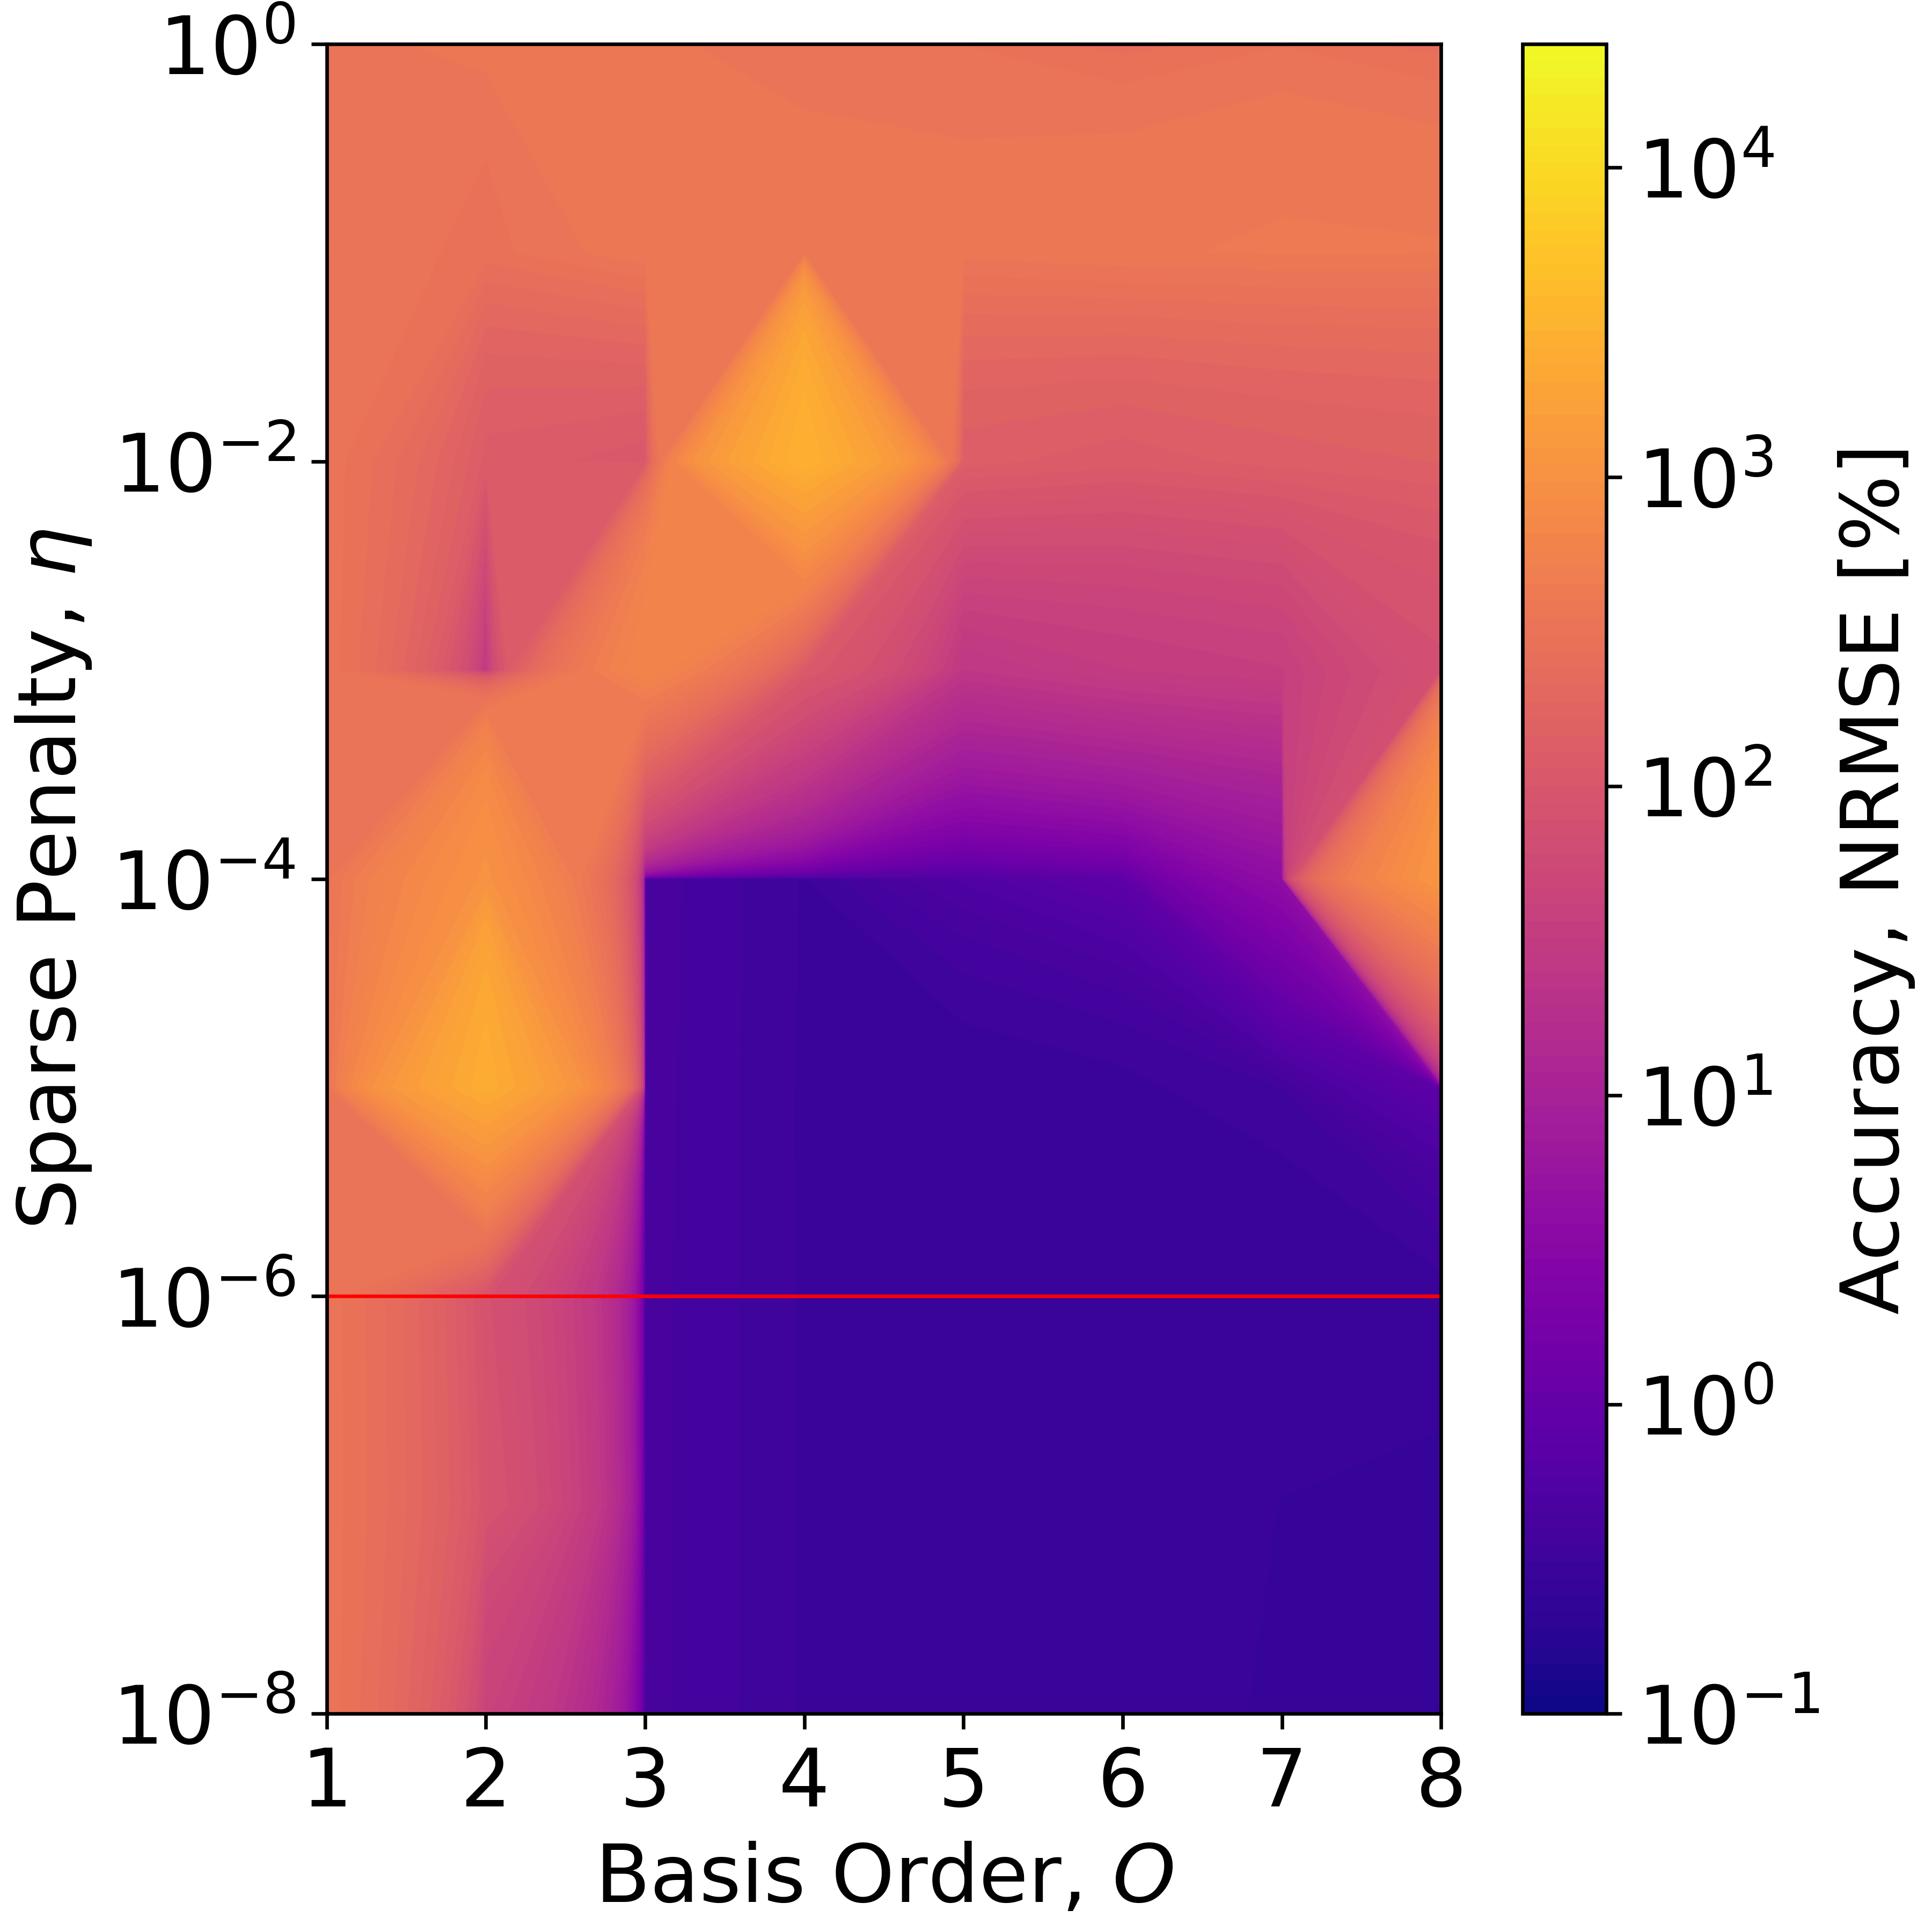
\includegraphics[width=0.99\textwidth]{../figs/guidance/value_function_nrmse.png}
                \end{figure}
            \end{graybox}}
        \end{column}
        \begin{column}{0.33\textwidth}
            \visible<3->{
            \begin{graybox}{Cardinality}
                \centering
                \begin{figure}
                    \centering
                    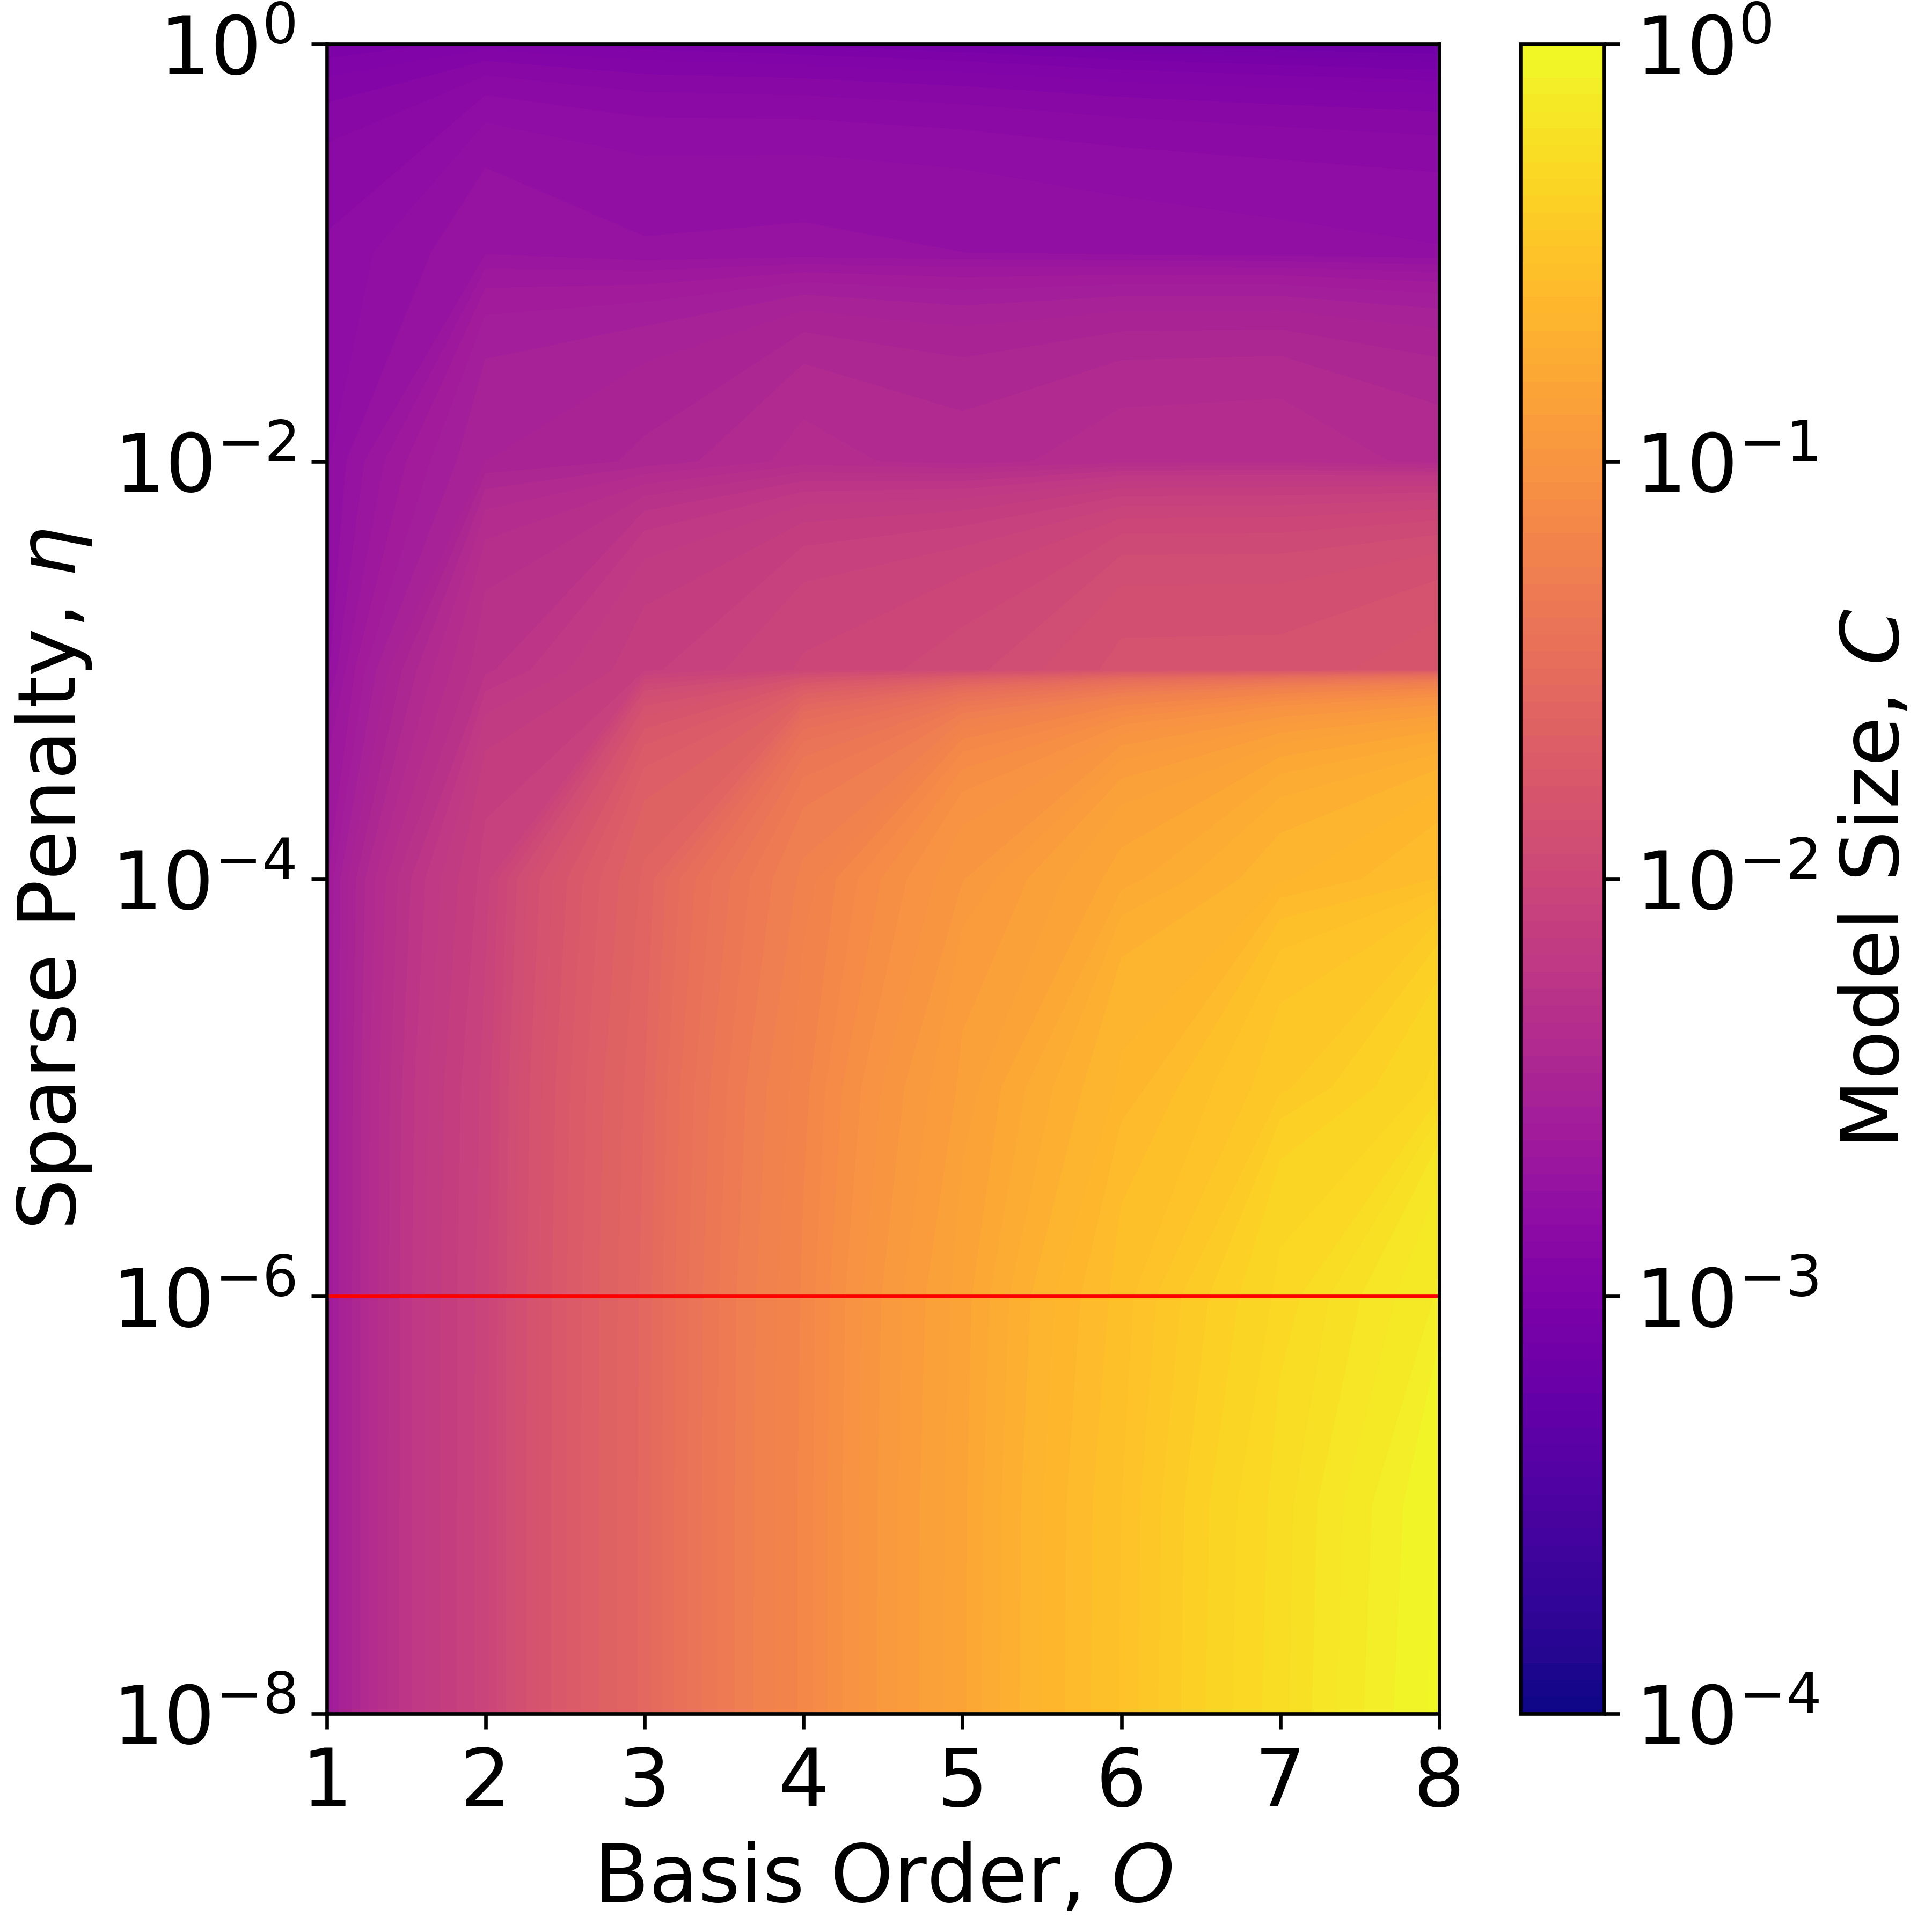
\includegraphics[width=0.99\textwidth]{../figs/guidance/value_function_cardinality.png}
                \end{figure}
            \end{graybox}}
        \end{column}
        \begin{column}{0.33\textwidth}
            \visible<4->{
            \begin{graybox}{Trade-Off}
                \centering
                \begin{figure}
                    \centering
                    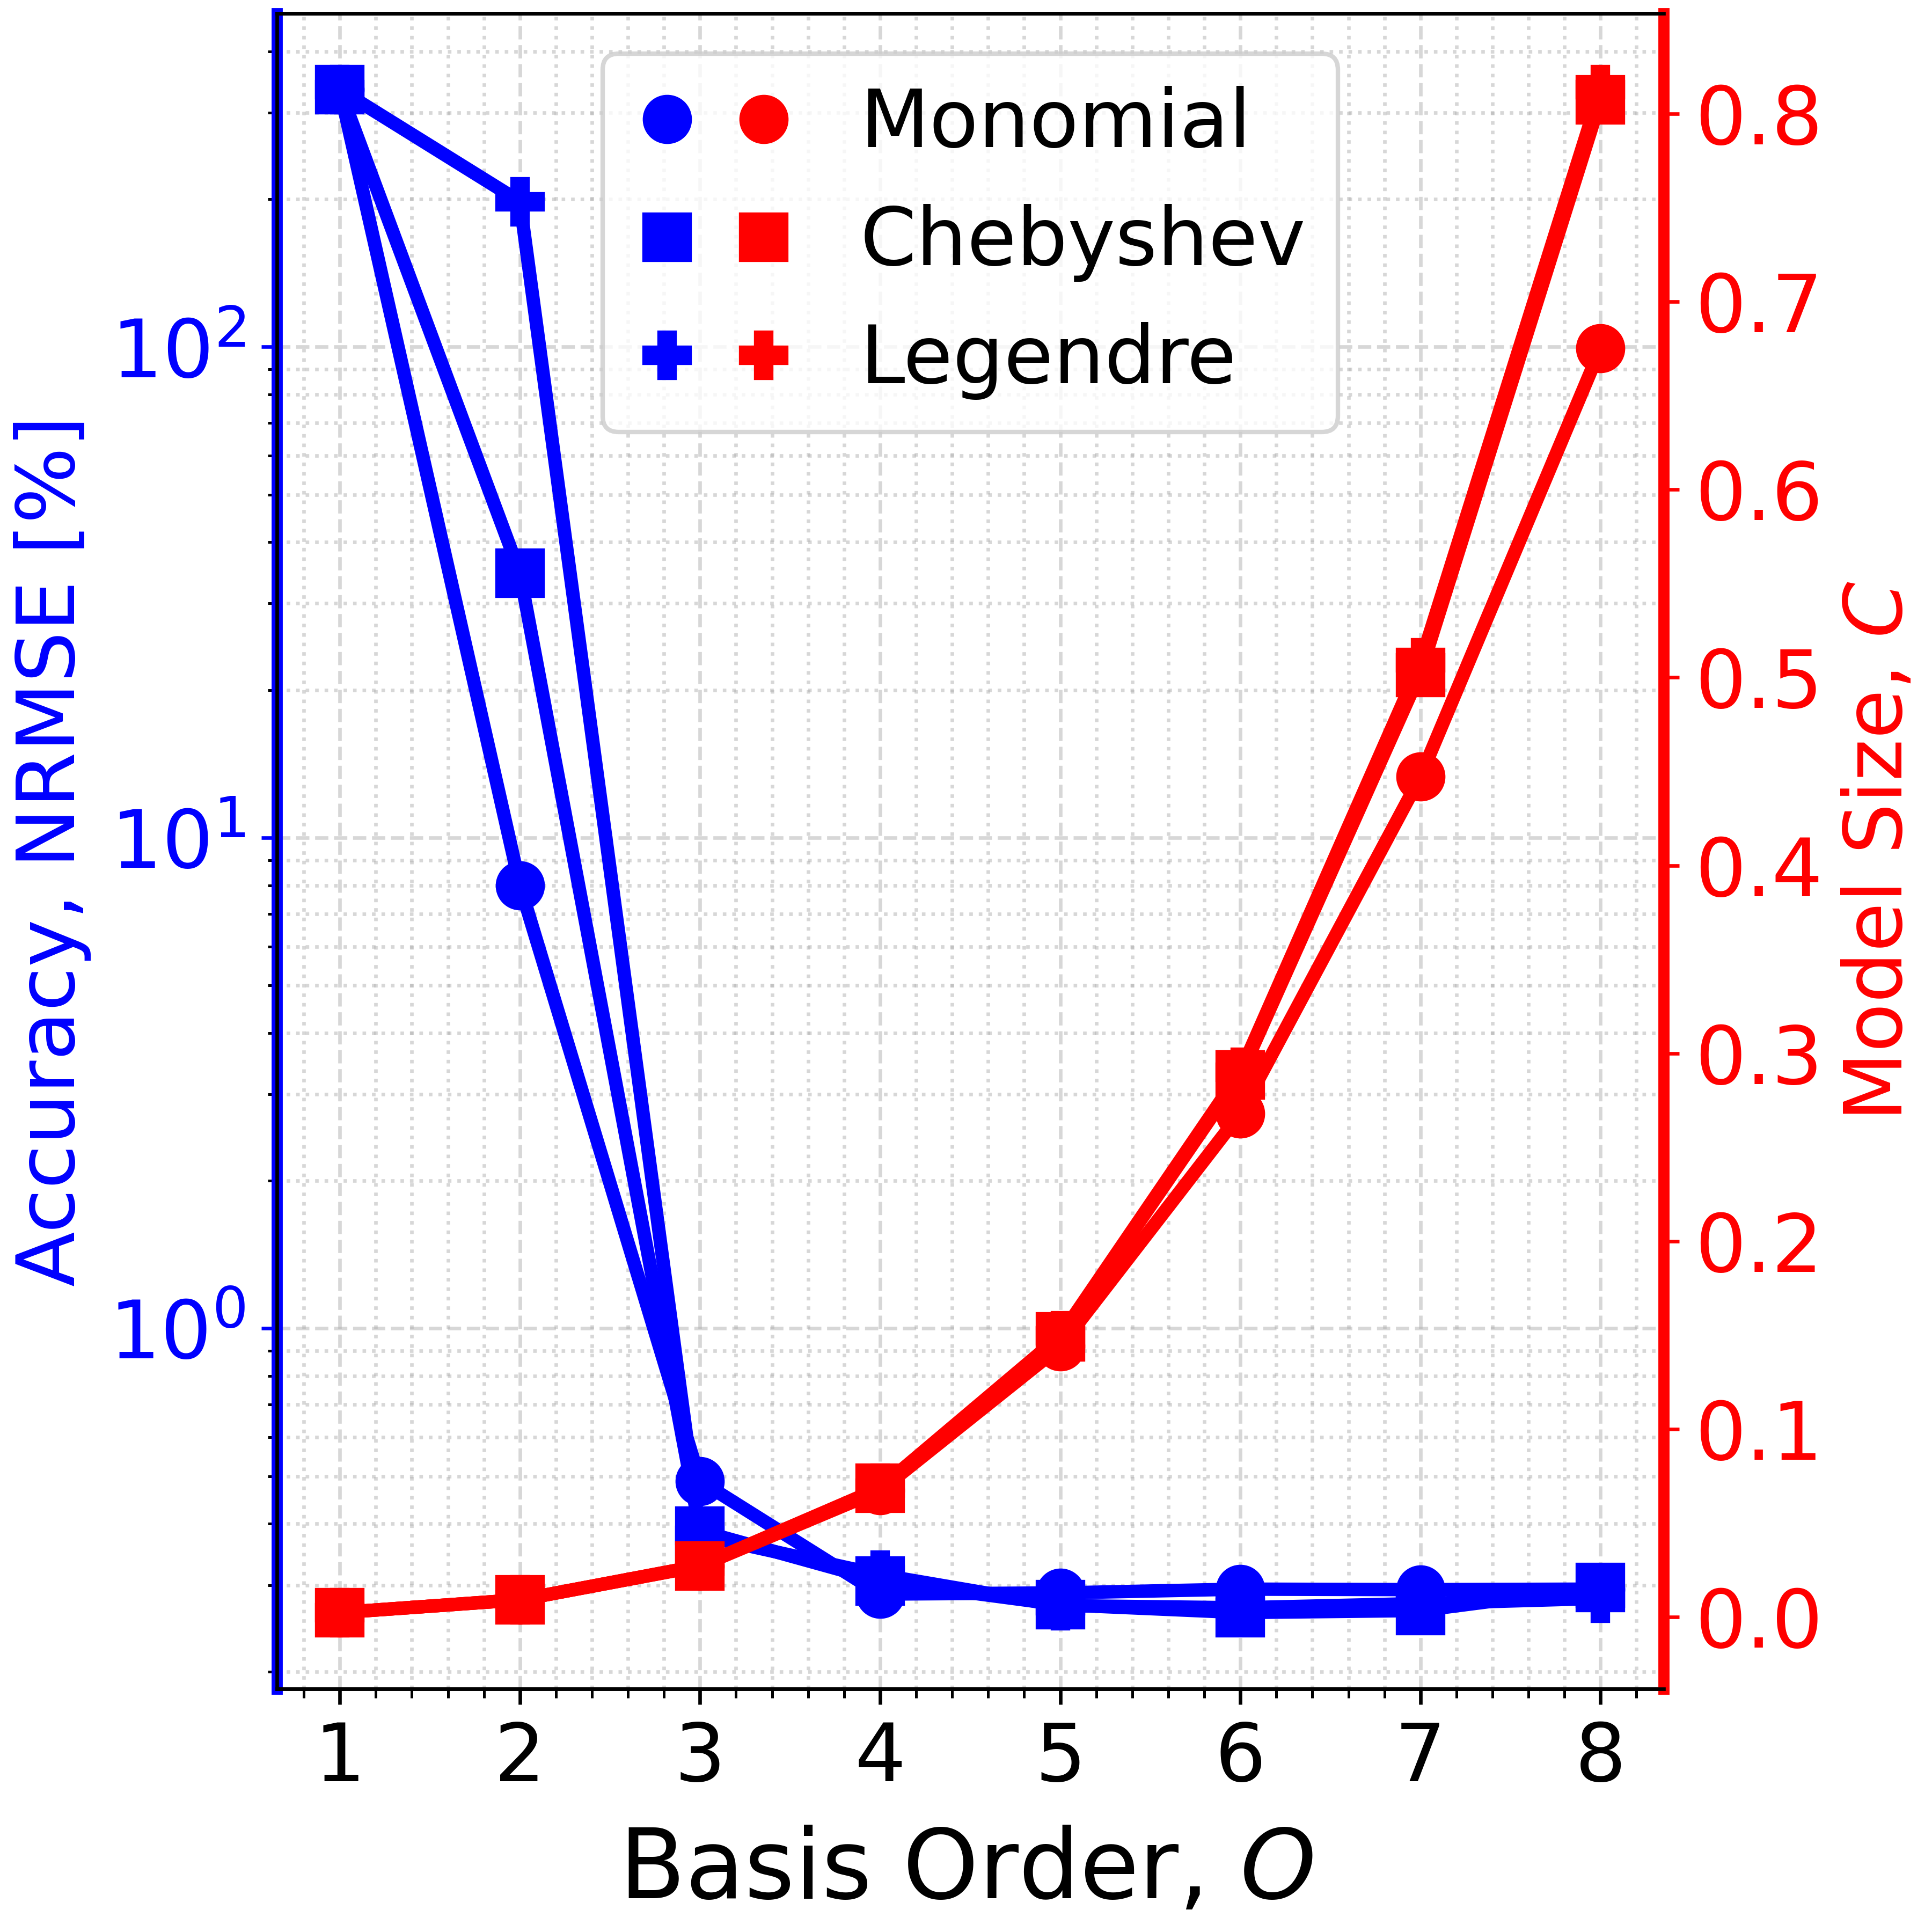
\includegraphics[width=0.99\textwidth]{../figs/guidance/value_function_tradeoff.png}
                \end{figure}
            \end{graybox}}
        \end{column}
    \end{columns}
    \begin{center}
        {\tiny 
        $\eta$: sparse penalty, $O$: basis order, $m$: basis cardinality}
    \end{center}
\end{frame}

\begin{frame}{Numerical Results: Trajectory Optimization}
    \footnotesize
    \visible<1->{Maximal \textbf{terminal velocity}  at a \textbf{specified target} for hypersonic gliding system,}
    \begin{columns}
        \begin{column}{0.33\textwidth}
            \visible<2->{
            \begin{graybox}{Closed-Loop Simulations}
                \begin{figure}
                    \centering
                    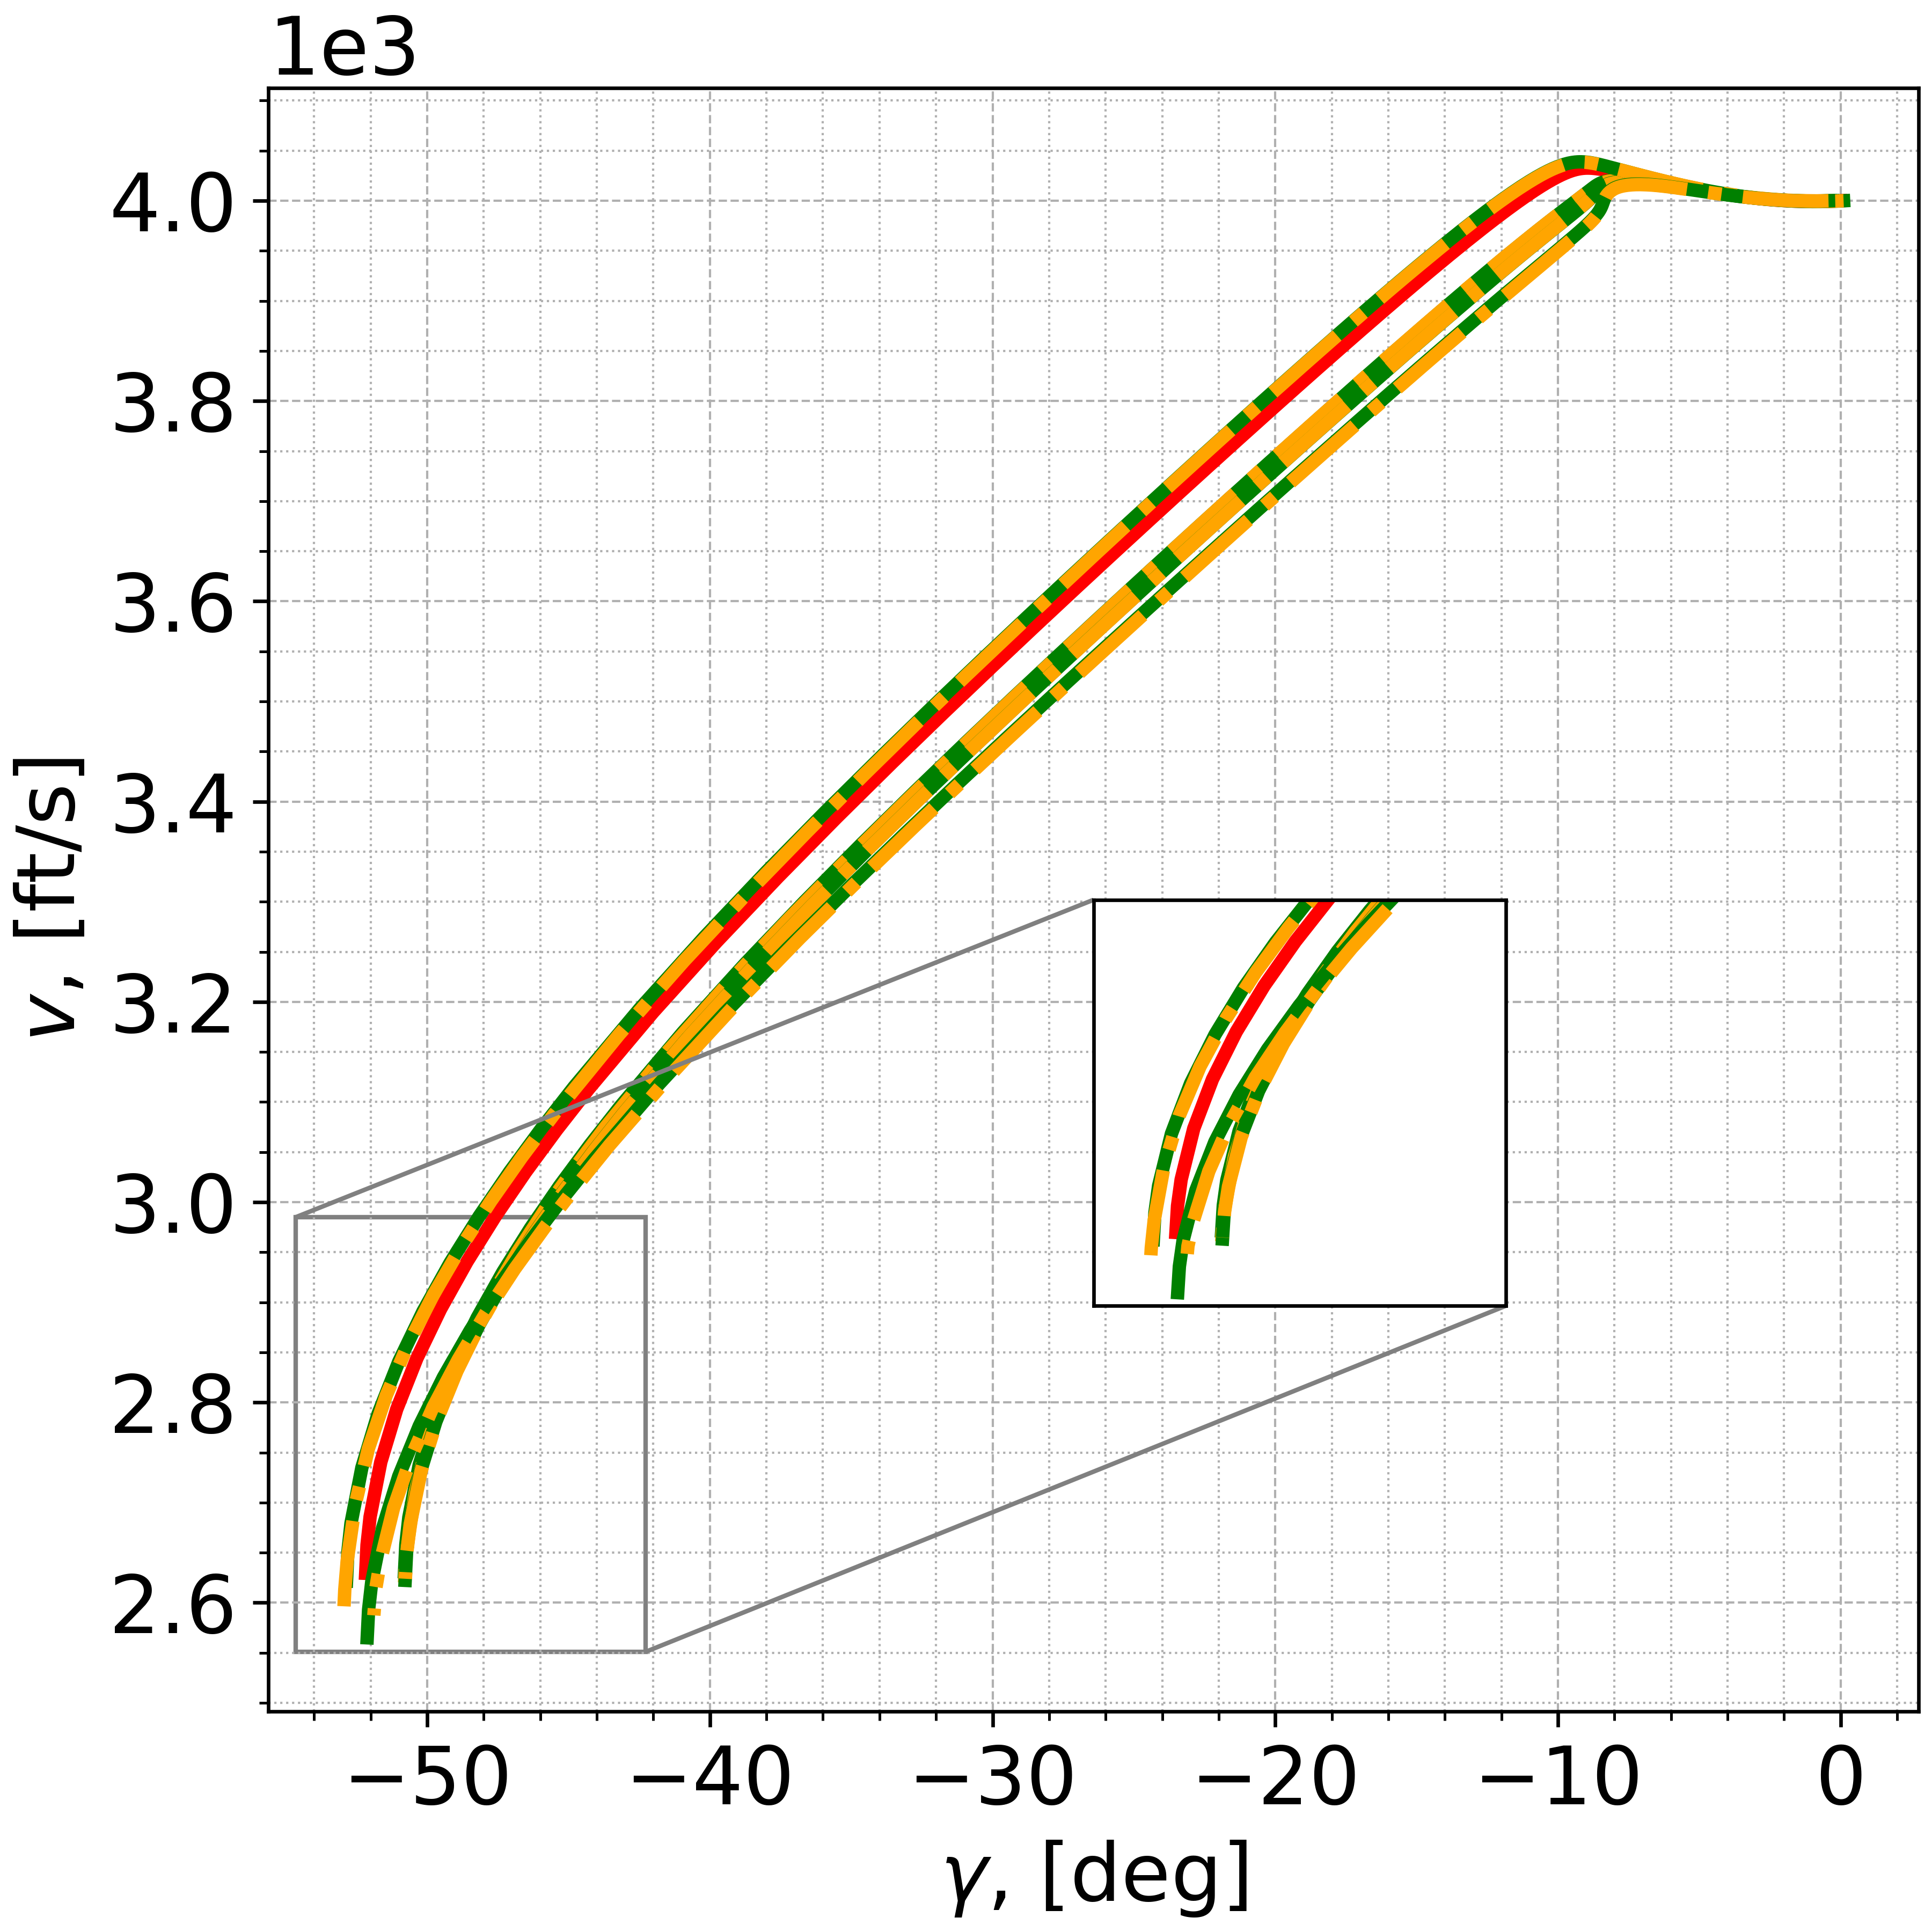
\includegraphics[width=0.9\textwidth]{../figs/guidance/planar_hypersonic_vg_2.png}
                \end{figure}
            \end{graybox}}
        \end{column}
        \begin{column}{0.33\textwidth}
            \visible<3->{
            \begin{graybox}{Boundary Perturbations}
                \begin{figure}
                    \centering
                    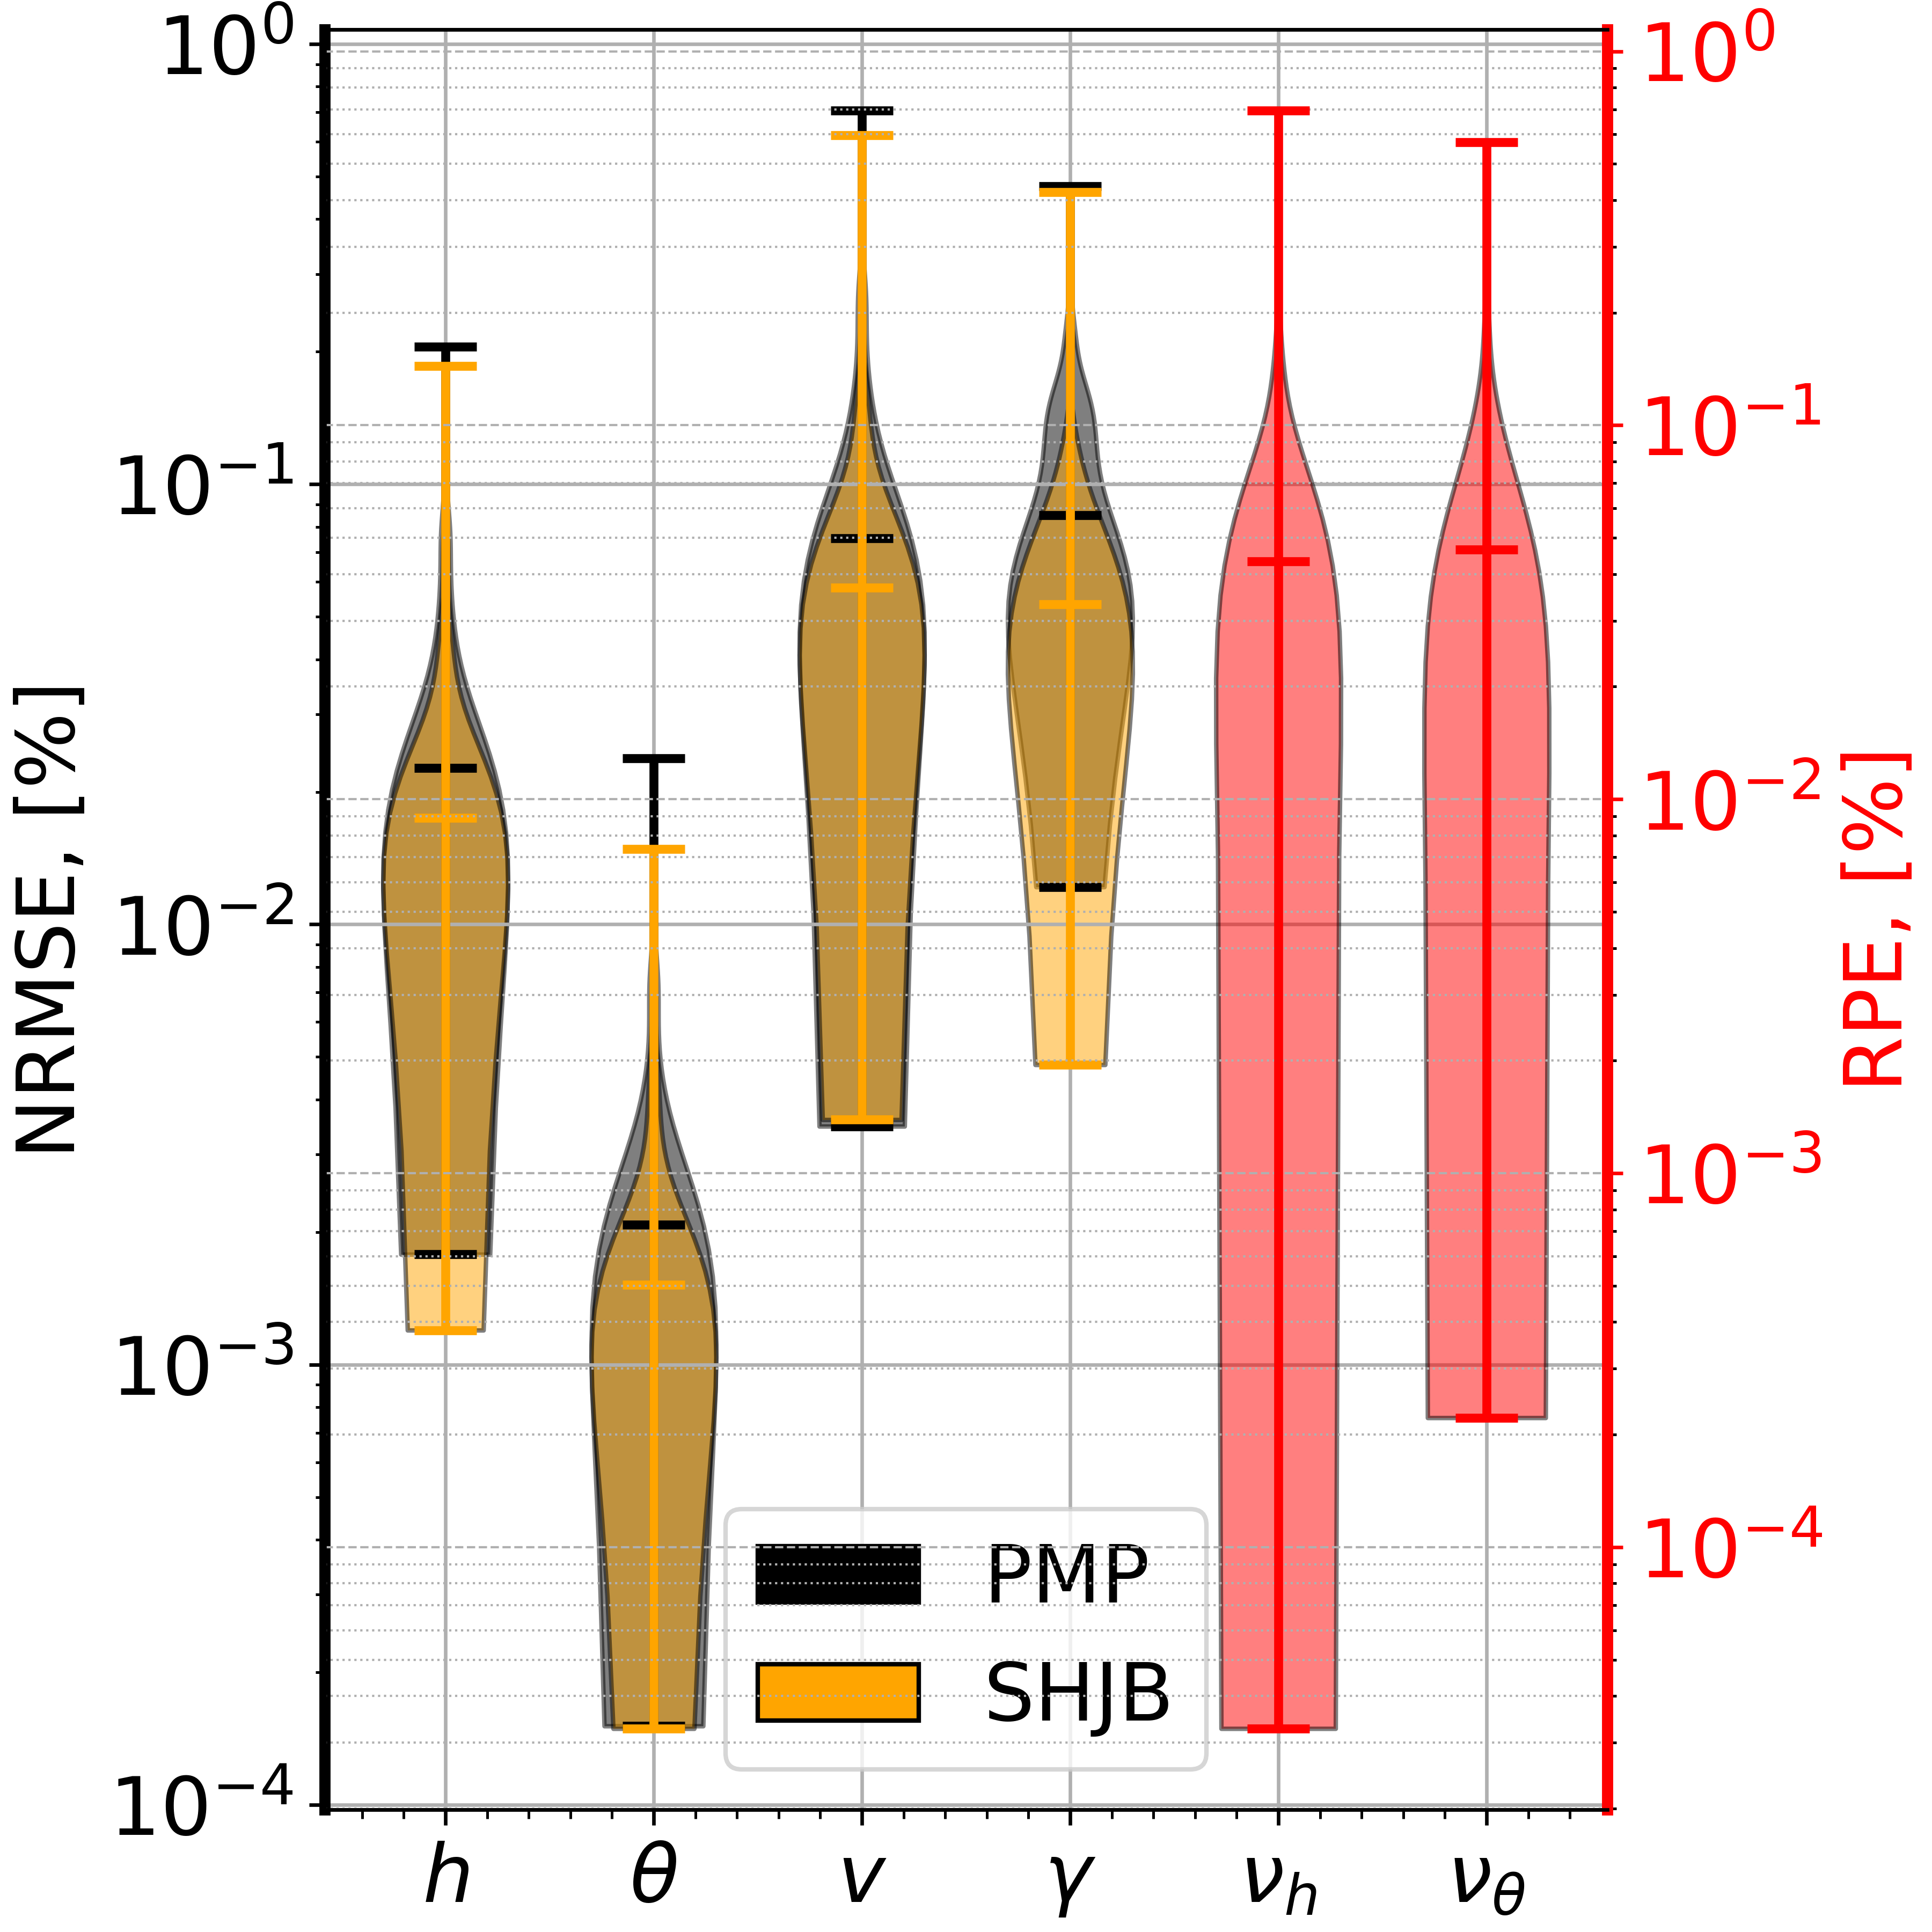
\includegraphics[width=0.9\textwidth]{../figs/guidance/planar_hypersonic_errors_1.png}
                \end{figure}
            \end{graybox}}
        \end{column}
        \begin{column}{0.33\textwidth}
            \visible<4->{
            \begin{graybox}{Model Peturbations}
                \begin{figure}
                    \centering
                    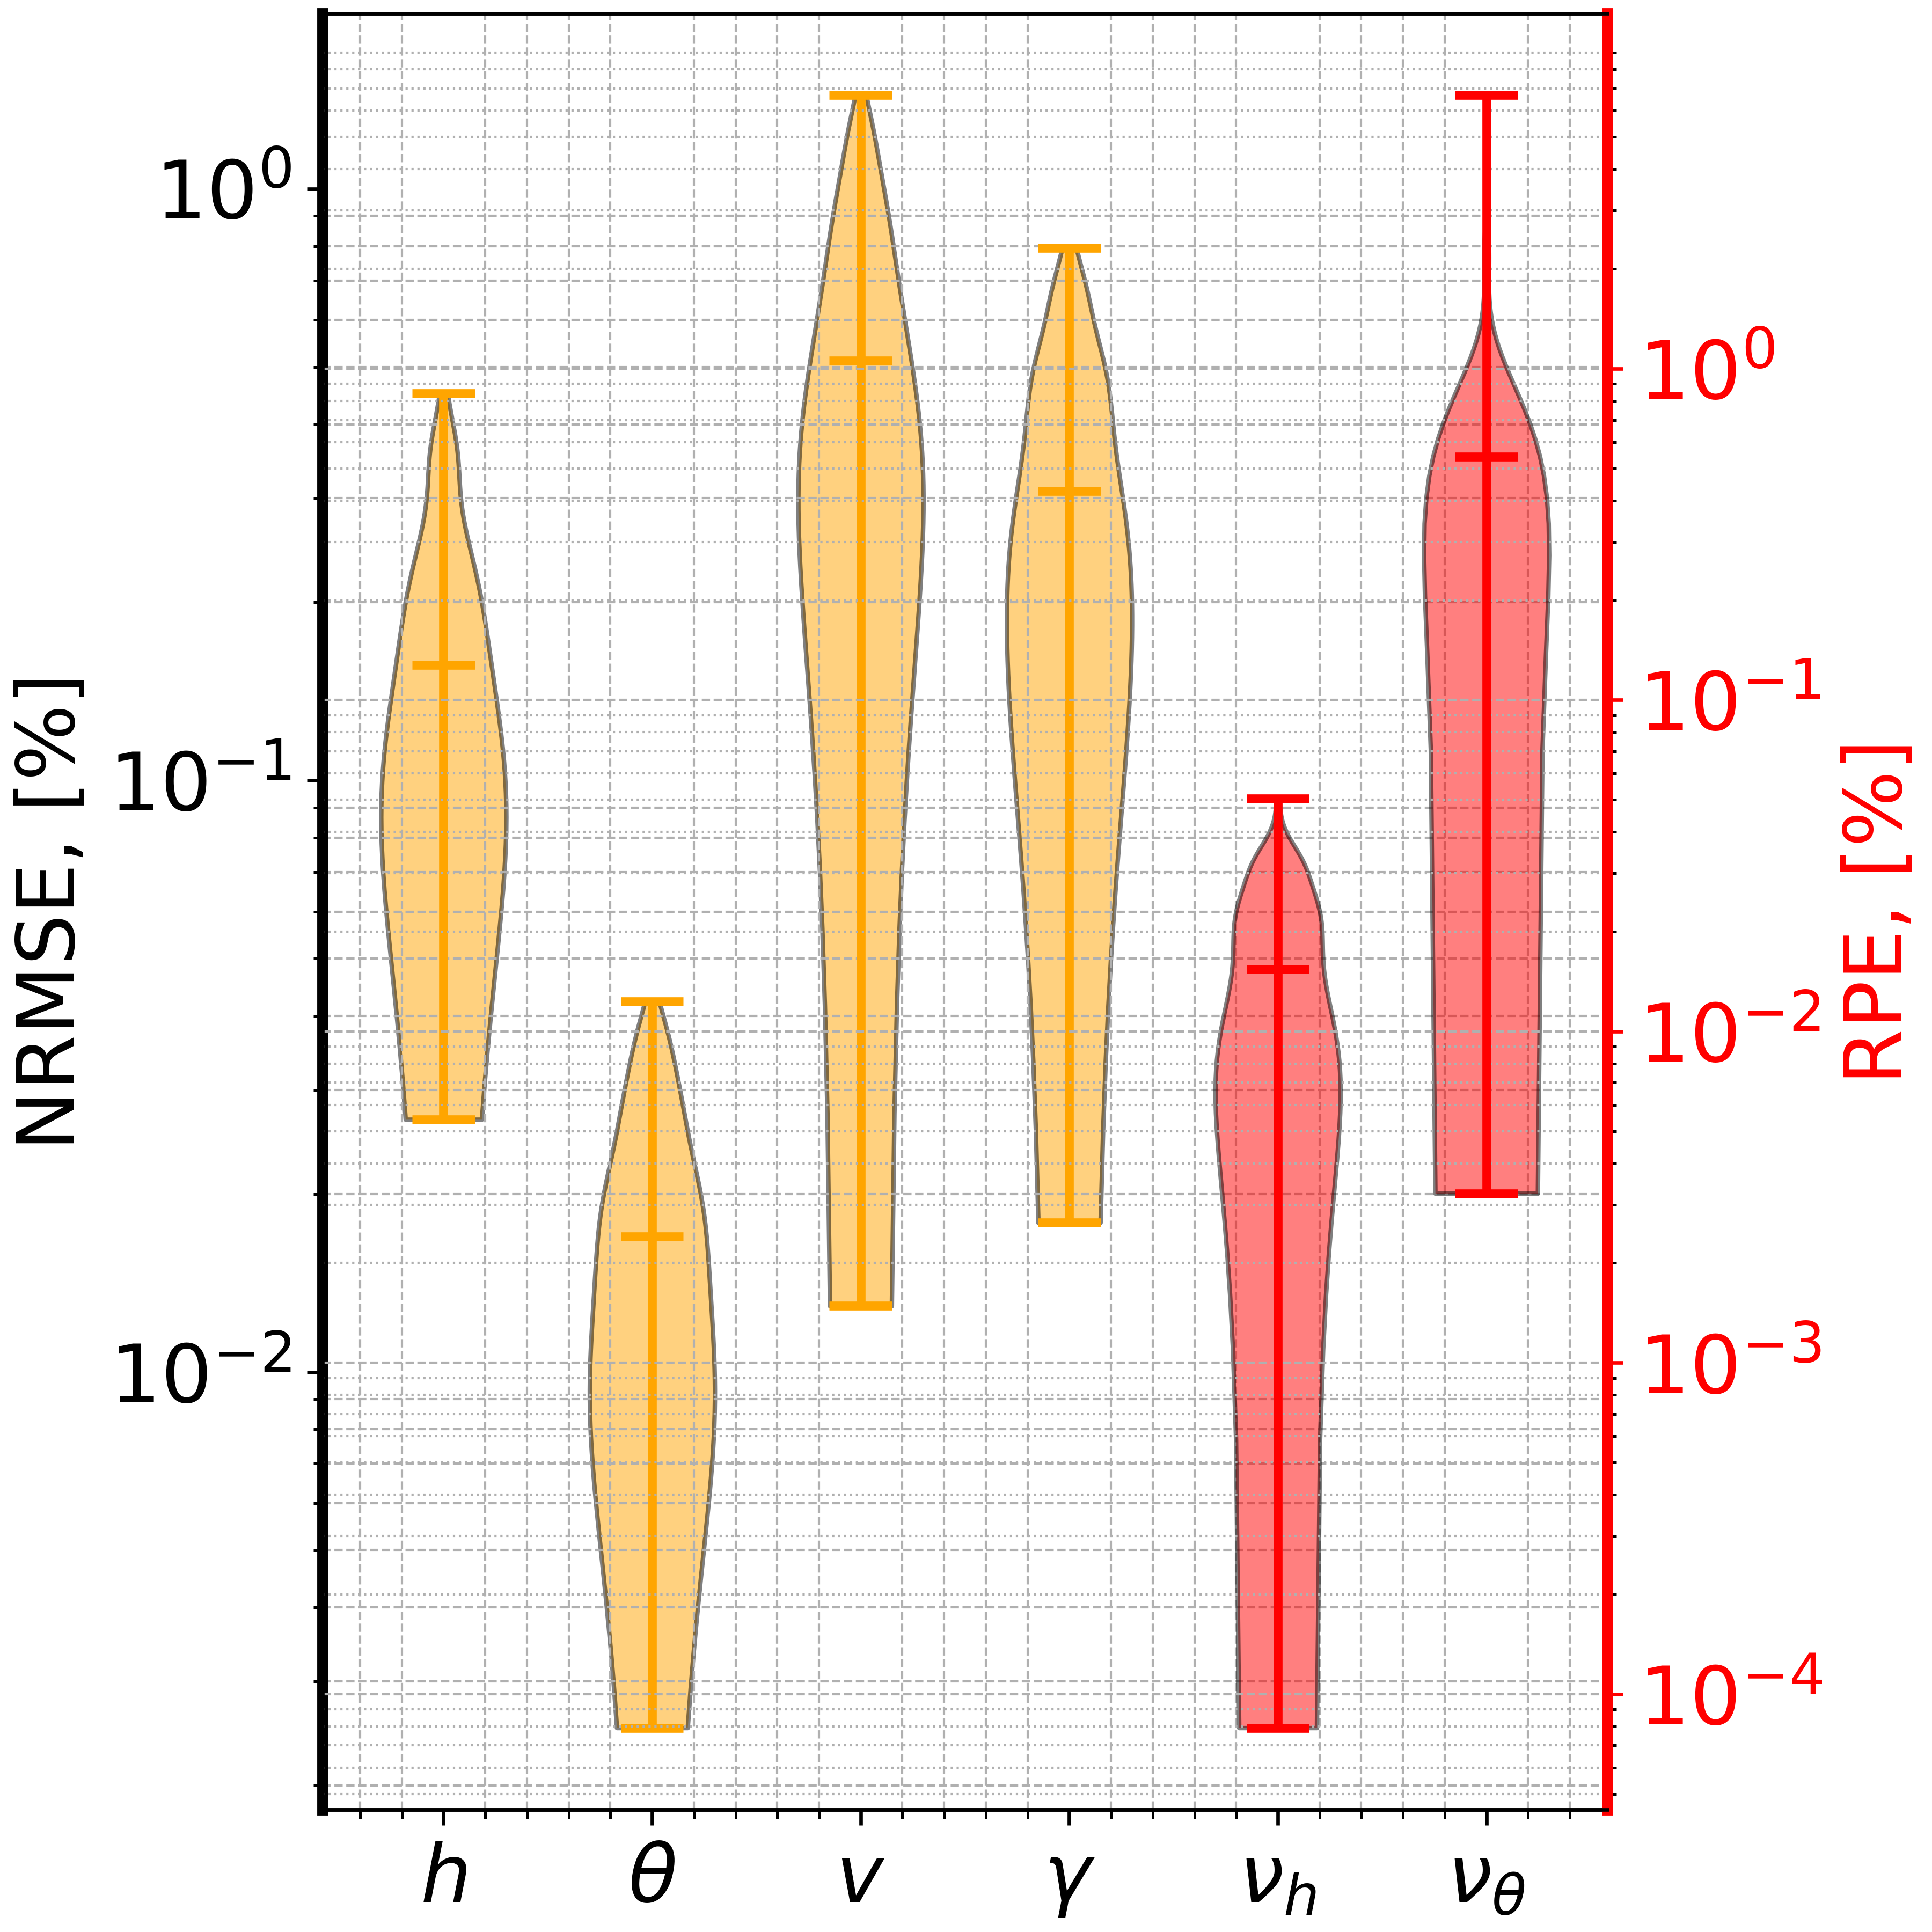
\includegraphics[width=0.9\textwidth]{../figs/guidance/planar_hypersonic_errors_2.png}
                \end{figure}
            \end{graybox}}
        \end{column}
    \end{columns}
    \begin{center}
        {\tiny 
        $h$: altitude, $v$: velocity, $\gamma$: flight-path angle, $\theta$: longitude, $\nu_h$: altitude terminal sensitivity, $\nu_\theta$: terminal longitude sensitivity
        }
    \end{center}
\end{frame}

\begin{frame}{Numerical Results: Trajectory Optimization}
    \footnotesize
    \visible<1->{Space shuttle re-entry \textbf{cross-range} maximization,}
    \begin{columns}
        \begin{column}{0.33\textwidth}
            \visible<2->{
            \begin{graybox}{Closed-Loop Simulation}
                \begin{figure}
                    \centering
                    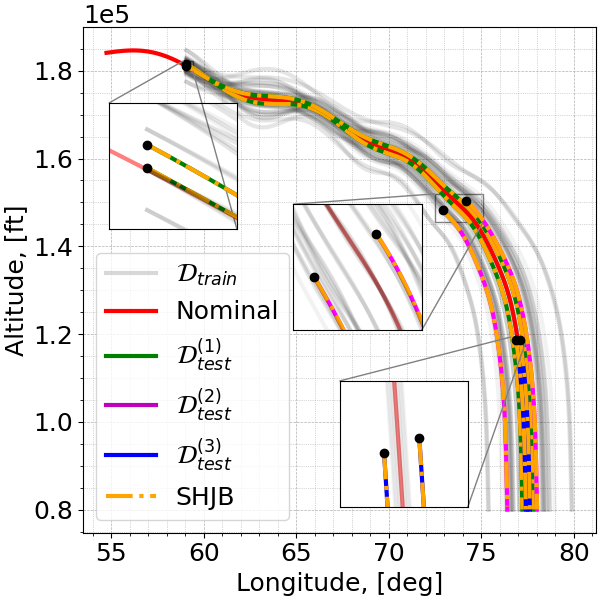
\includegraphics[width=0.99\textwidth]{../figs/guidance/space_shuttle_altitude_simulation.png}
                \end{figure}
            \end{graybox}}
        \end{column}
        \begin{column}{0.33\textwidth}
            \visible<3->{
            \begin{graybox}{Performance Comparison}
                \begin{figure}
                    \centering
                    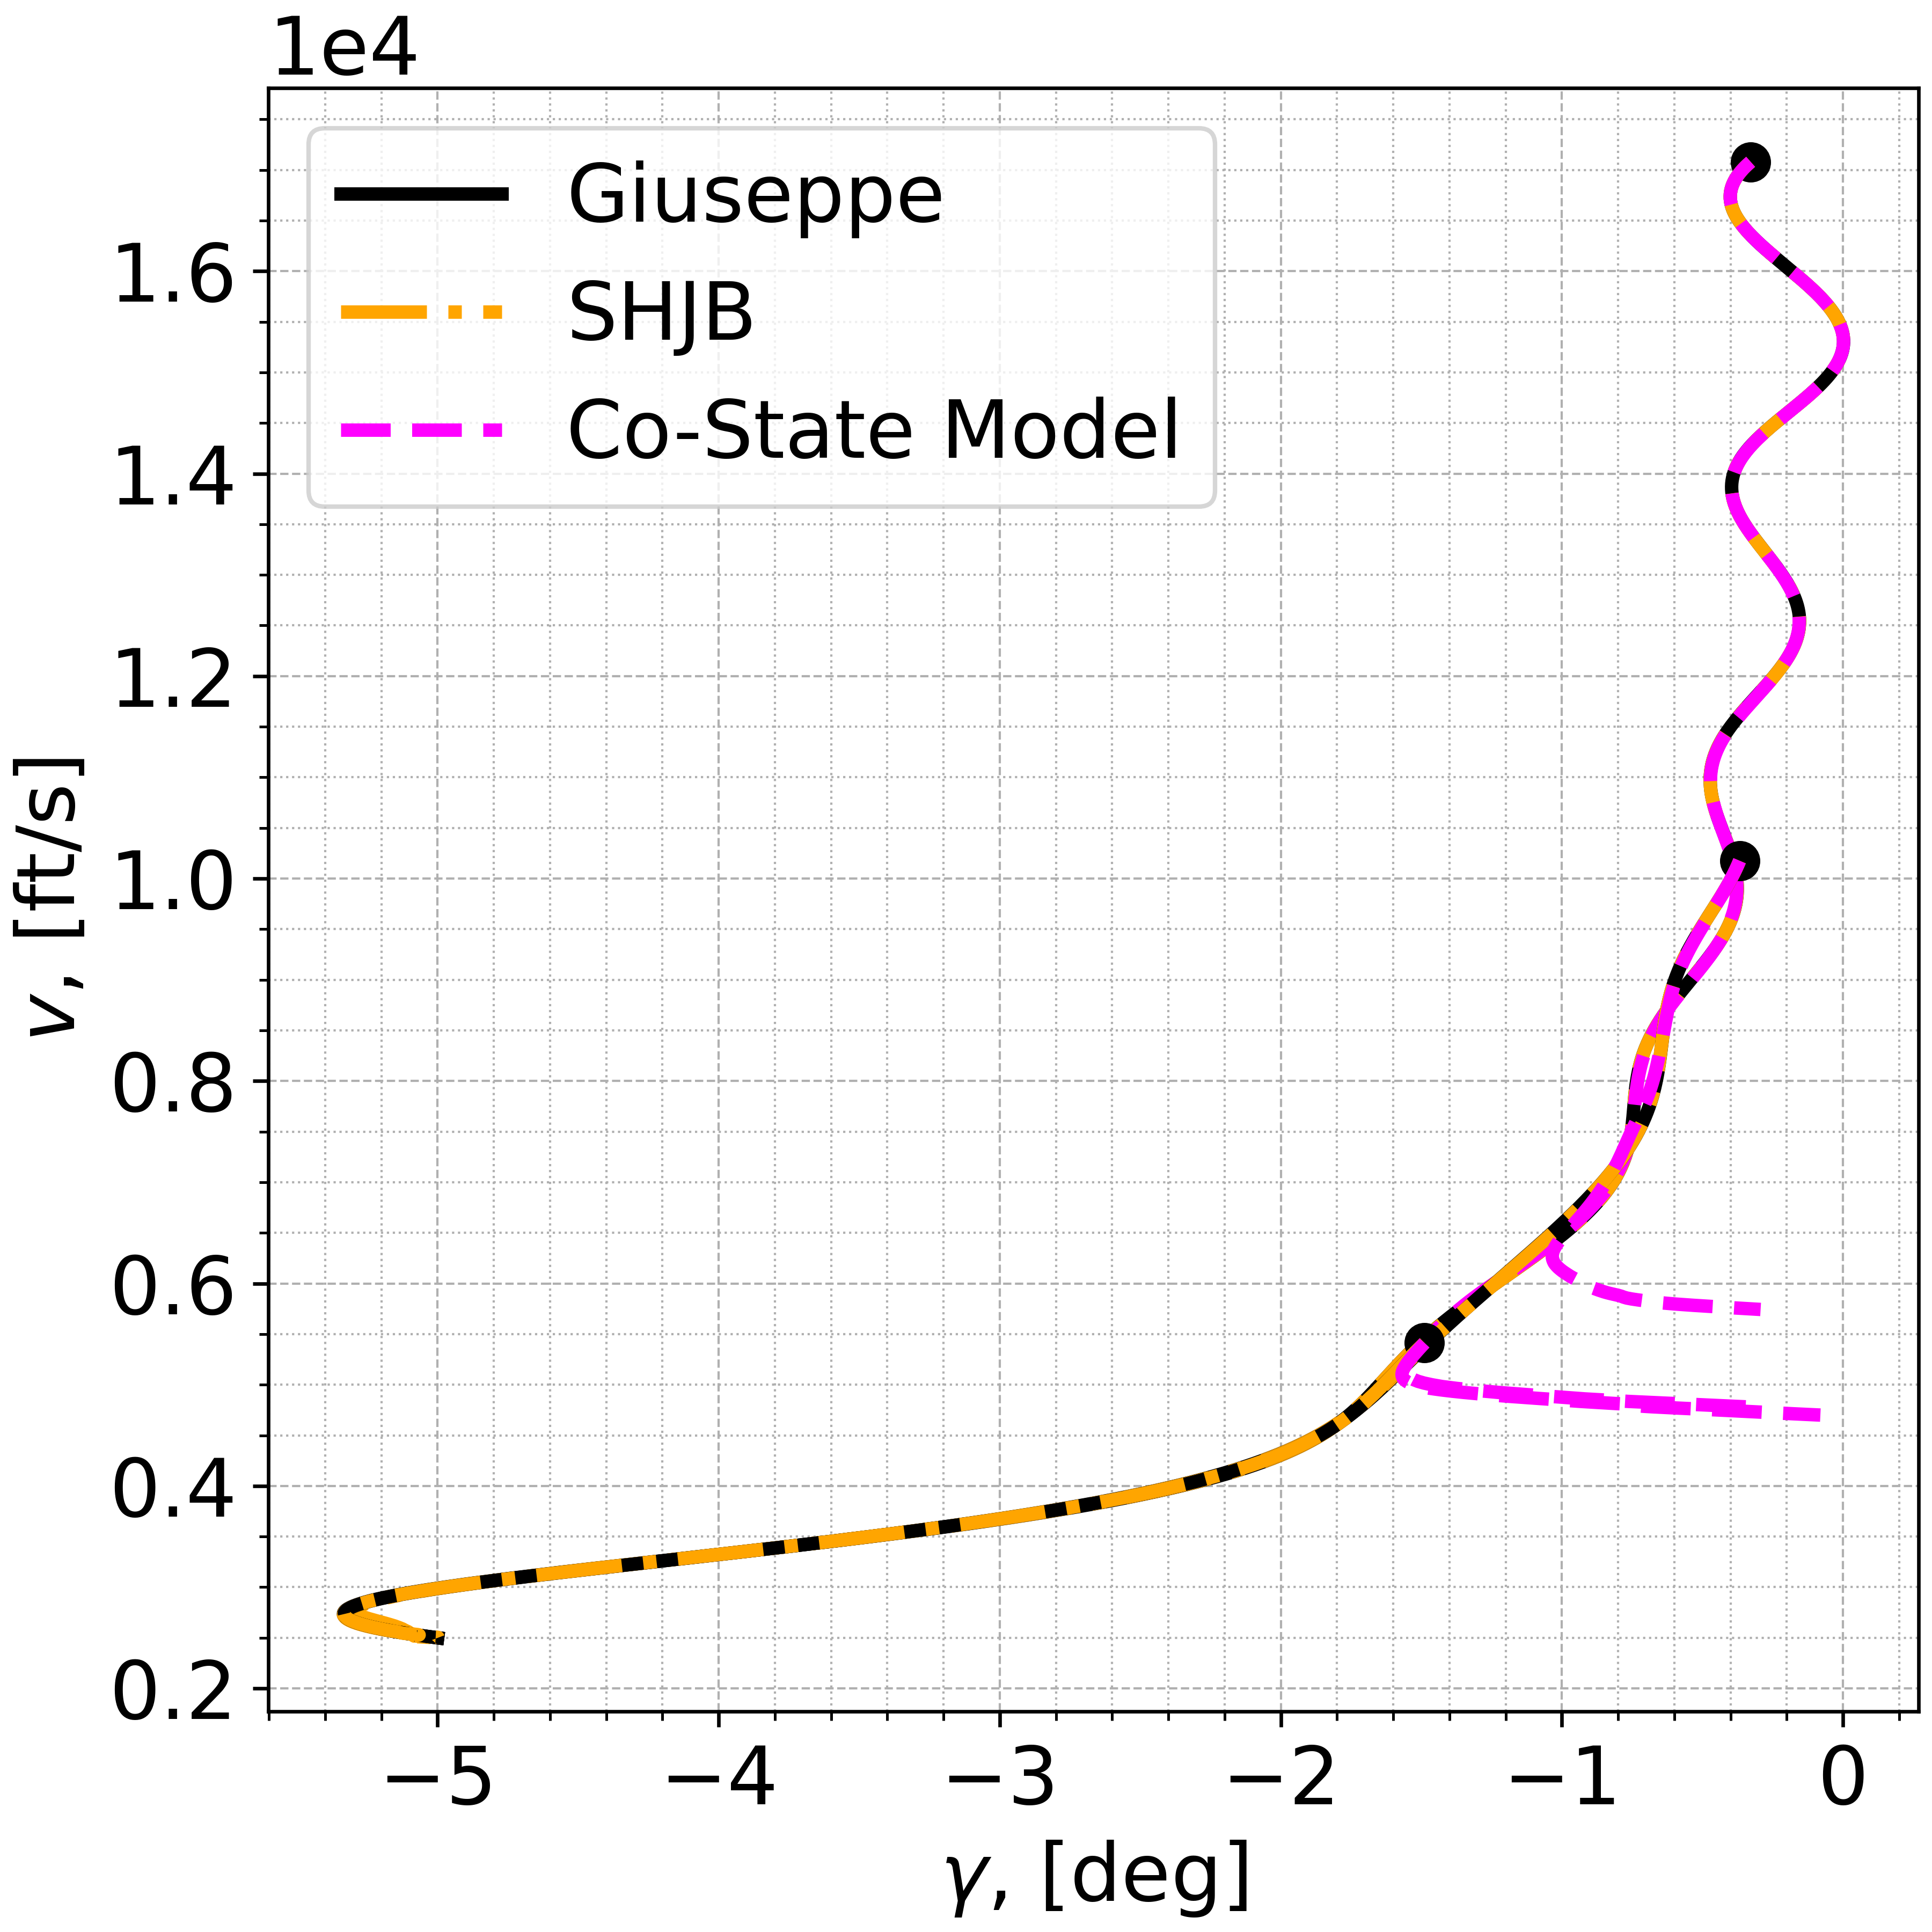
\includegraphics[width=0.99\textwidth]{../figs/guidance/space_shuttle_pi_vs_pmp_velocity_vs_fpa.png}
            \end{figure}
            \vspace*{-0.2in}
            \centering
            {\tiny \textbf{improved generalizability!}}
            \end{graybox}}
        \end{column}
        \begin{column}{0.33\textwidth}
            \visible<4->{
            \begin{graybox}{Boundary Perturbations}
                \begin{figure}
                    \centering
                    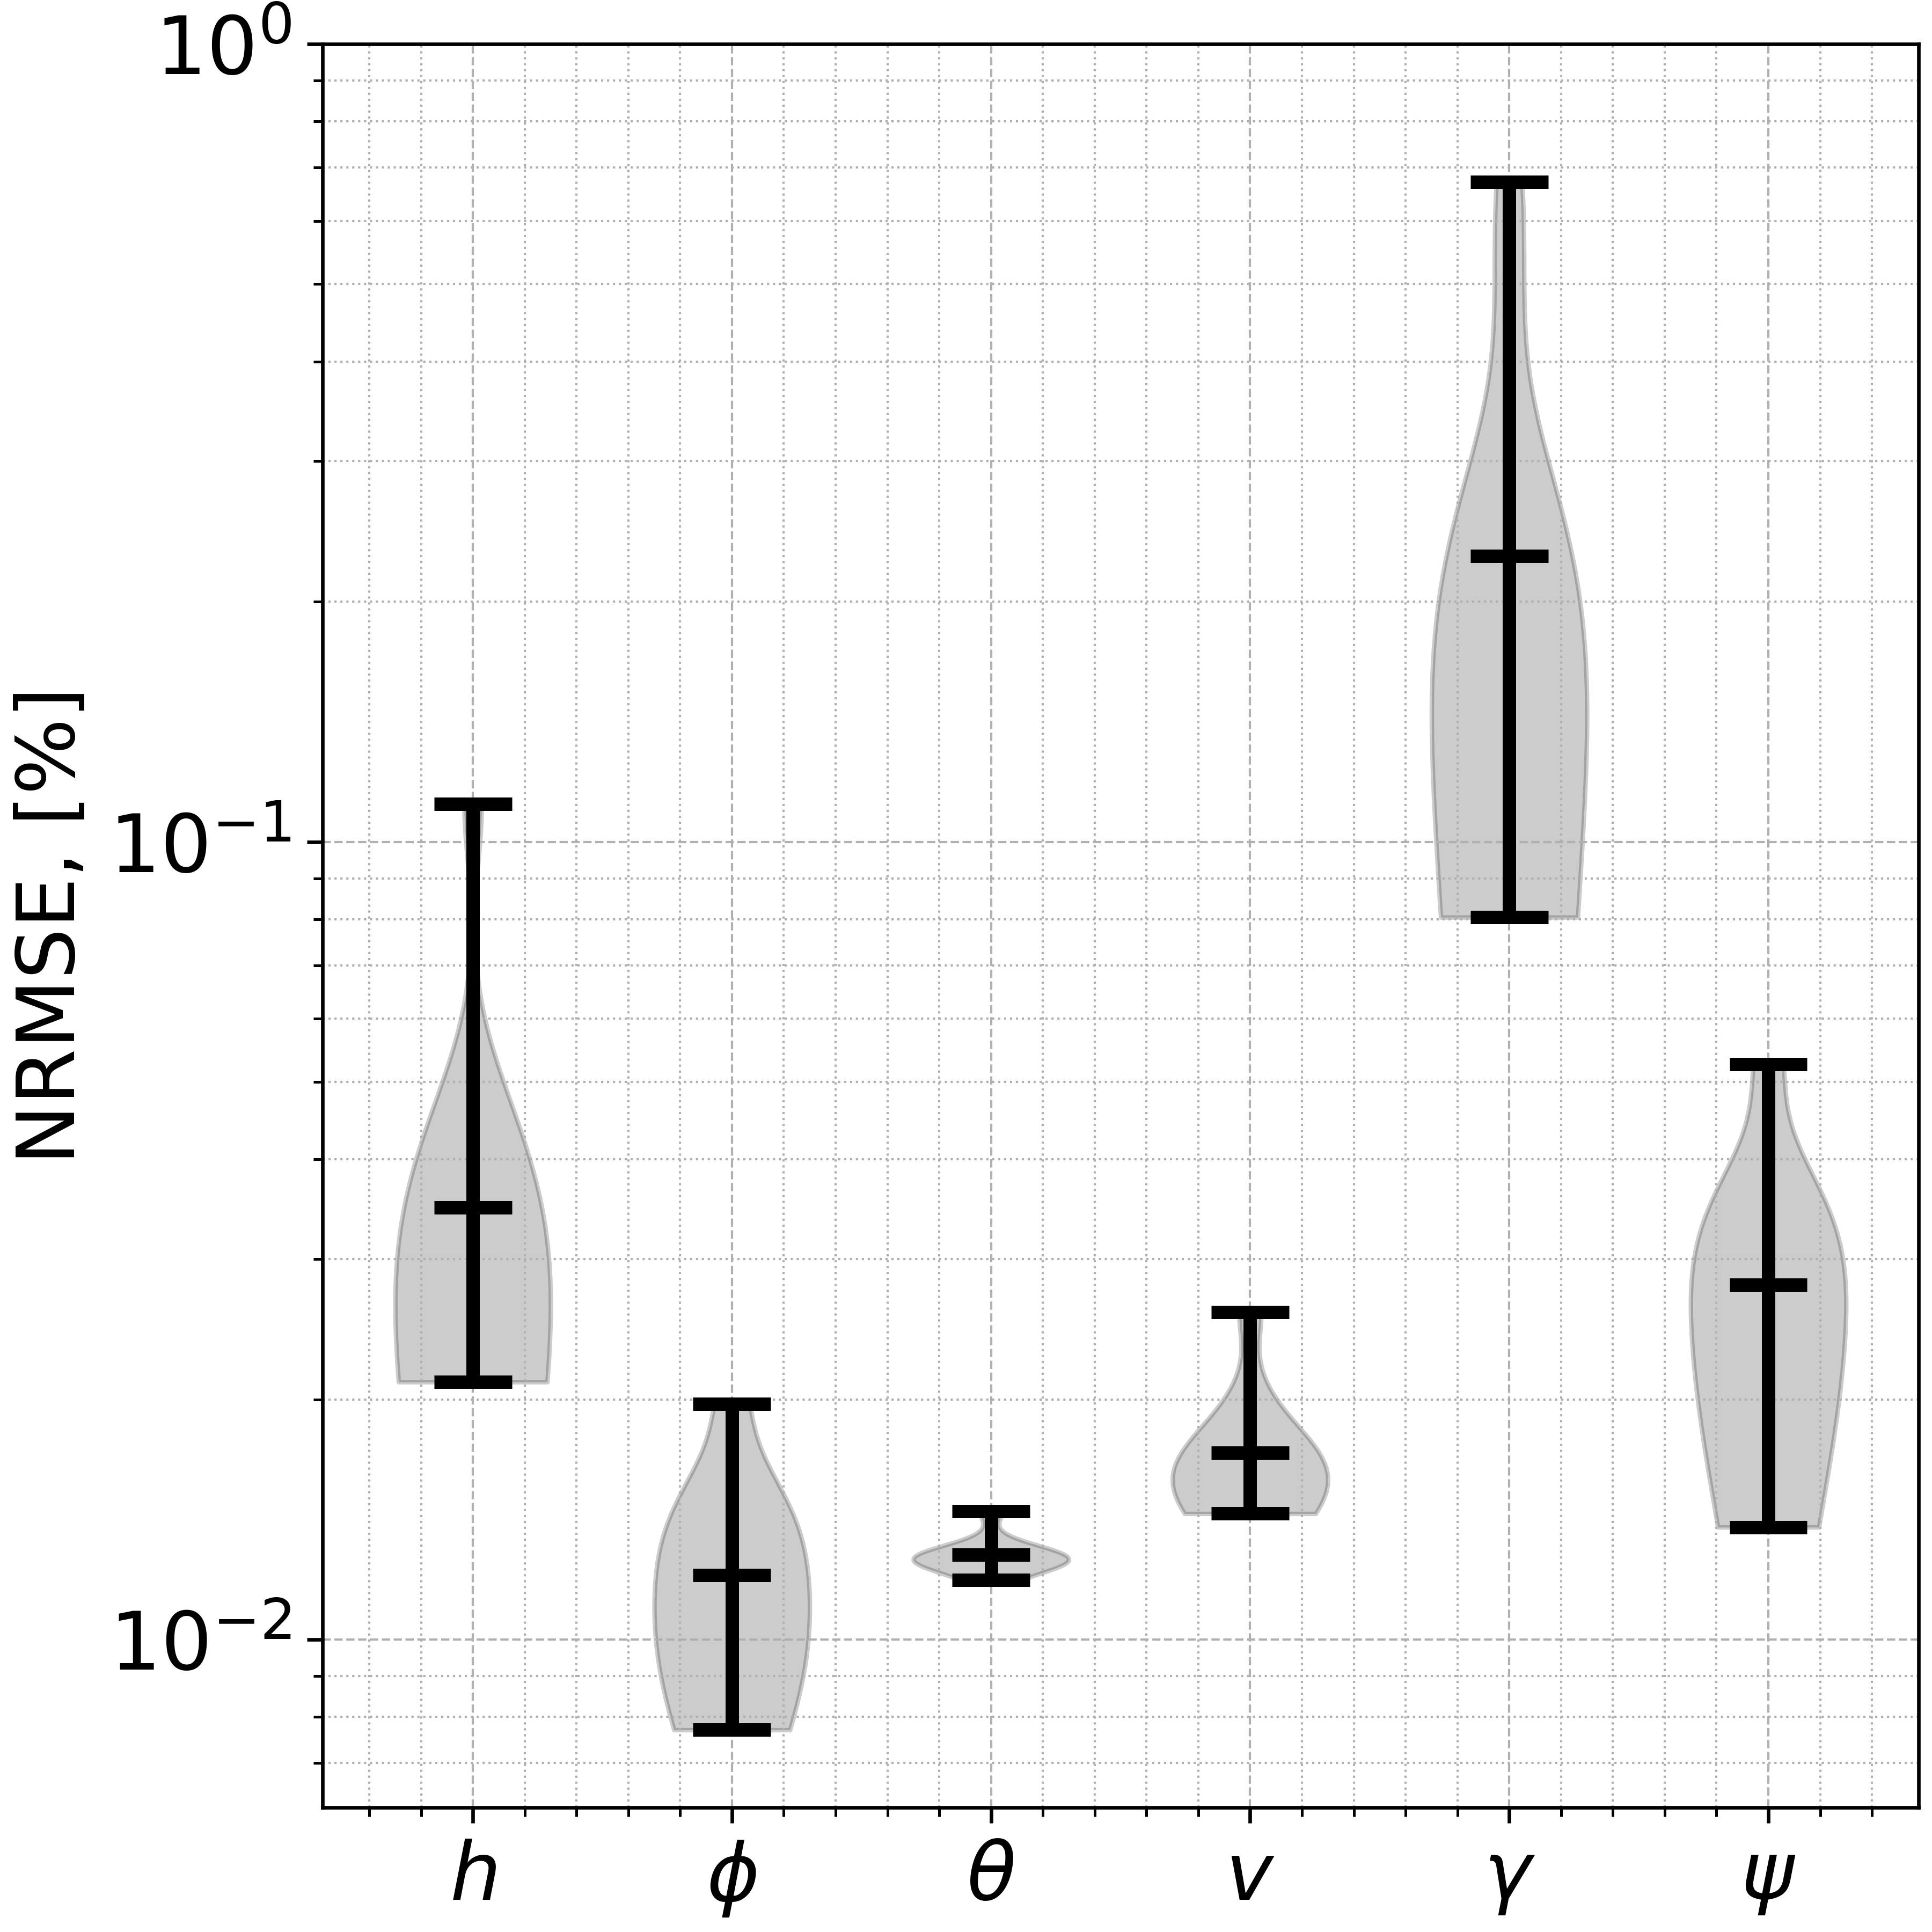
\includegraphics[width=0.99\textwidth]{../figs/guidance/simulation_errors.png}
                \end{figure}
            \end{graybox}}
        \end{column}
    \end{columns}
    \begin{center}
        {\tiny
        SHJB: Sparse Hamilton-Jacobi-Bellman, $h$: altitude, $v$: velocity, $\gamma$: flight-path angle, $\theta$: longitude, $\phi$: latitude, $\psi$: heading
        }
    \end{center}
\end{frame}

\begin{frame}{Numerical Results: Trajectory Optimization}
    \footnotesize
    \begin{columns}
        \begin{column}{0.4\textwidth}
            \centering
            \visible<1->{
            \textbf{Is the ITOC solved?}
            \begin{figure}
                \centering
                
\includegraphics[width=0.9\textwidth]{../../Chapter-1/Figures/itoc.png}
            \end{figure}}
        \end{column}
        \begin{column}{0.7\textwidth}
            \centering
            \begin{itemize}
                \item<2-> \textbf{Accuracy}: comparable to indirect OCP solutions (NRMSE $<1\%$)
                \item<3-> \textbf{Efficiency}:
                \begin{itemize}
                    \item<4-> \textbf{Online}: $\mathcal{A}\approx 10^3 - 10^4$ and $\cC\approx 0.2$
                    \item<4-> \textbf{Offline}: not quantified (on-going work)
                \end{itemize}
                \item<5-> \textbf{Generalizability}: accurate for unseen BCs and model parameters 
                \begin{center}
                    (\textcolor{red}{but no guarantees outside the tube!})
                \end{center}        
            \end{itemize}
        \end{column}
    \end{columns}
    \visible<2->{
    \begin{tikzpicture}[remember picture, overlay]
        \node[anchor=north west, xshift=2.2cm, yshift=-2.8cm] at (current page.north west) {
\includegraphics[width=0.1\textwidth]{../figs/pirom/checkmark.png}};
    \end{tikzpicture}}
    \visible<3->{
    \begin{tikzpicture}[remember picture, overlay]
        \node[anchor=north west, xshift=0.1cm, yshift=-5.8cm] at (current page.north west) {
\includegraphics[width=0.08\textwidth]{../figs/pirom/exclamation.png}};
    \end{tikzpicture}}
    \visible<5->{
    \begin{tikzpicture}[remember picture, overlay]
        \node[anchor=north west, xshift=4.45cm, yshift=-5.8cm] at (current page.north west) {
\includegraphics[width=0.1\textwidth]{../figs/pirom/checkmark.png}};
    \end{tikzpicture}}
\end{frame}